% @Author:  Youssef Ayadi
% @Project: SIPMS — Smart Internship and Project Management System
% @Company: CLINISYS
% @Year:    2024/2025

\documentclass[12pt, oneside, a4paper]{Configuration/IIT-report}

\graphicspath{{images/}}

%%%%%%%%%%%%%%%%%%%%%%%%%%%%%%%%%%%%%%%%%%%%%%%%%%%%%%%%%%%
% Include useful commands
%%%%%%%%%%%%%%%%%%%%%%%%%%%%%%%%%%%%%%%%%%%%%%%%%%%%%%%%%%%
\newcommand{\reportAuthor} {%
  Prénom \textsc{NOM}%
}

\newcommand{\reportTitle} {%
   TITRE DU PROJET \\ Title%
}

\newcommand{\reportSubject} {%
   TITRE DU PROJET \\ Title%
}

\newcommand{\dateSoutenance} {%
  jj/mm/aaaa%
}

\newcommand{\studyDepartment} {%
  Génie Systèmes Électroniques 
et Communication%
}

\newcommand{\codePFE} {% Reference %
}

\newcommand{\juryPresident} {%
  Mr Foulen \textsc{Fouleni}%
}
\newcommand{\juryPresidentDesc} {%
  President%
}

\newcommand{\juryMemberOne} {%
  Ms Foulena \textsc{Foulenia}%
}
\newcommand{\juryMemberOneDesc} {%
  Supervisor %Mentor
}

\newcommand{\juryMemberTwo} {%
  Mr Foulen \textsc{Fouleni}%
}
\newcommand{\juryMemberTwoDesc} {%
  Reviewer% Examiner, Reporter
}

\newcommand{\specialcell}[1]{%
  \begin{tabularx}{\textwidth}{@{}X@{}}#1\end{tabularx}%
}

%%%%%%%%%%%%%%%%%%%%%%%%%%%%%%%%%%%%%%%%%%%%%%%%%%%%%%%
% Add your own commands here
%%%%%%%%%%%%%%%%%%%%%%%%%%%%%%%%%%%%%%%%%%%%%%%%%%%%%%%
\newcommand{\MyCommand} {%
  Does nothing really%
}



\hypersetup{
  pdftitle={Smart Internship and Project Management System - SIPMS},%
  pdfauthor={Youssef Ayadi},%
  pdfsubject={Final Year Project — CLINISYS},%
  pdfkeywords={SIPMS} {internship} {management} {Spring Boot} {React} {AI} {IIT-Sfax}
}
\dominitoc
\begin{document}
    \thispagestyle{empty}
\definecolor{titleblue}{RGB}{0,82,155}
\definecolor{lineyellow}{RGB}{255,192,0}

\begin{tikzpicture}[remember picture,overlay]
    \node[inner sep=0pt] at (current page.center) {
\includegraphics[width=\paperwidth,height=\paperheight]{images/TemplateImages/page_background.jpeg}};
\end{tikzpicture}

\begin{titlepage}
\fontfamily{phv}\selectfont
\begin{center}

\begin{tabularx}{\textwidth}{@{} c >{\centering\arraybackslash}X c @{}}
  \begin{tabular}{c}
    
\includegraphics[width=2.2cm]{images/TemplateImages/coat_of_arms.png}\\[3pt]
    \textcolor{titleblue}{\fontsize{8pt}{10pt}\selectfont\textbf{Republic of Tunisia}}\\
    \textcolor{titleblue}{\fontsize{8pt}{10pt}\selectfont\textbf{Ministry of Higher Education}}\\
    \textcolor{titleblue}{\fontsize{8pt}{10pt}\selectfont\textbf{and Scientific Research}}
  \end{tabular}
  &
  \vspace{-10pt}
\includegraphics[width=1.8cm]{images/TemplateImages/tunisia_flag.png}
  &
  \vspace{-10pt}
\includegraphics[width=4.5cm]{images/TemplateImages/iit_full_logo.png}
\end{tabularx}

\vspace{35pt}
\textcolor{titleblue}{\fontsize{26pt}{30pt}\selectfont\textbf{GRADUATION PROJECT}}

\vspace{20pt}
\fontsize{12pt}{14pt}\selectfont\textbf{Performed at :}

\vspace{20pt}
\fontsize{12pt}{14pt}\selectfont Logo de la société

\vspace{30pt}
\fontsize{11pt}{13pt}\selectfont Elaborated by:

\vspace{5pt}
\fontsize{24pt}{28pt}\selectfont Full Name

\vspace{30pt}
\fontsize{11pt}{13pt}\selectfont In view of obtaining the National Diploma of 3 years bachelor in

\vspace{10pt}
\fontsize{14pt}{18pt}\selectfont\textbf{COMPUTER SCIENCES}

\vspace{20pt}
\fontsize{11pt}{13pt}\selectfont Entitled :

\vspace{10pt}
\setlength{\fboxrule}{0.75pt}
\fcolorbox{lineyellow}{white}{
  \parbox{0.9\textwidth}{
    \centering
    \vspace{15pt}
    \fontsize{22pt}{26pt}\selectfont\textbf{PROJECT TITLE}
    \vspace{15pt}
  }
}

\vspace{20pt}
\fontsize{11pt}{13pt}\selectfont Defended on : D/M/2026

\vspace{5pt}
Committee :

\vspace{10pt}
\begin{tabular}{l @{\hspace{20pt}} l}
  Mr. Full Name & --\hspace{10pt}Chairman \\
  Mr. Full Name & --\hspace{10pt}Examiner \\
  Mr. Full Name & --\hspace{10pt}Academic supervisor \\
  Mr. Full Name & --\hspace{10pt}Industrial supervisor \\
\end{tabular}

\vfill

\textcolor{titleblue}{\fontsize{11pt}{13pt}\selectfont\textbf{ACADEMIC YEAR : 2025-2026}}

\vspace{10pt}

\end{center}
\end{titlepage}

    
    % Page numbering
    \pagenumbering{arabic}
    \doublespacing{}
    
    % Dedication
    \chapter*{DEDICATION}
%\addstarredchapter{DEDICATION}
%\addcontentsline{toc}{chapter}{DEDICATION}
%\adjustmtc
\thispagestyle{MyStyle}
%
%For all they have endured to satisfy all my needs and wishes
\begin{center}
À Lorem ipsum dolor sit amet, consectetur adipiscing elit. Sed non risus. Suspendisse lectus tortor, dignissim sit amet, adipiscing nec, ultricies sed, dolor. Cras elementum ultrices diam. Maecenas ligula massa, varius a, semper congue, euismod non, mi. \\
\textbf{À mon cher, Prenom}.\\
À Lorem ipsum dolor sit amet, consectetur adipiscing elit. Sed non risus. Suspendisse lectus tortor, dignissim sit amet, adipiscing nec, ultricies sed, dolor. Cras elementum ultrices diam.\\ 
\textbf{À ma chère, Prenom}.\\
À Lorem ipsum dolor sit amet, consectetur adipiscing elit. Sed non risus. Suspendisse lectus tortor, dignissim sit amet, adipiscing nec, ultricies sed, dolor. Cras elementum ultrices diam. Maecenas ligula massa, varius a, semper congue, euismod non, mi. \\
\textbf{À mon cher, Prenom}.\\
\end{center}
\nopagebreak{%
  \raggedright\hspace{5.75cm} \textbf{ À vous tous},~\\
  \raggedright\hspace{7.75cm} Je dédie ce travail\@.~\\~\\~\\
  \vspace{-2cm}
  \raggedleft\normalfont\large\itshape{} \reportAuthor\par%
}

    % Acknowledgements
    % ============================================================
%   ACKNOWLEDGEMENTS
% ============================================================
\chapter*{ACKNOWLEDGEMENTS}
\markboth{\MakeUppercase{Acknowledgements}}{}
\addcontentsline{toc}{chapter}{Acknowledgements}
\thispagestyle{MyStyle}

\par
First and foremost, I would like to express my deepest gratitude to \textbf{Allah} for granting me the strength, patience, and perseverance to complete this work.

\par
I would like to express my deepest gratitude to my academic supervisor, \textbf{Mrs. Rahma Bouaziz}, for her invaluable guidance, constructive feedback, and continuous support. I am also profoundly thankful to my industrial supervisor, \textbf{Mr. Marwen Hadrich}, for his mentorship, expertise, and for welcoming me into \textbf{CLINISYS}.

\par
I would also like to extend my sincere thanks to the Committee President, \textbf{Mr. Fahmi Kallel}, and to the honorable Reviewer for accepting to evaluate this work. Their insights and expertise are highly appreciated.

\par
I extend my sincere thanks to the entire team at \textbf{CLINISYS} for welcoming me into their organization and providing an enriching and stimulating professional environment. Their collaboration and trust were essential to the success of this project.

\par
My heartfelt appreciation goes to the faculty and staff of \textbf{IIT Sfax} for the quality education and technical training they have provided throughout my studies. The knowledge and skills acquired during my academic journey have been the foundation upon which this project was built.

\par
I am also deeply grateful to my family, whose love, encouragement, and sacrifices have sustained me throughout my academic career. A special thank you to my friends and colleagues for their moral support and camaraderie.

\par
Finally, I wish to thank all those who, directly or indirectly, contributed to the completion of this project.

\vspace{1cm}
\begin{flushright}
\textbf{Youssef Ayadi}
\end{flushright}

    % TABLE OF CONTENTS & LIST OF FIGURES
    \addtocontents{toc}{\protect\thispagestyle{MyStyle}}
        \renewcommand*\contentsname{TABLE OF CONTENTS}
        \begin{spacing}{1}
            \tableofcontents
        \end{spacing}
        \addtocontents{lof}{\protect\thispagestyle{MyStyle}}
        \renewcommand{\listfigurename}{LIST OF FIGURES}
        \begin{spacing}{1}
            \listoffigures
        \end{spacing}
        \addcontentsline{toc}{chapter}{\listfigurename}
        \adjustmtc

    % Abbreviations
    % ============================================================
%   ABBREVIATIONS LIST
% ============================================================
\chapter*{LIST OF ABBREVIATIONS}
\markboth{\MakeUppercase{List of Abbreviations}}{}
\addcontentsline{toc}{chapter}{List of Abbreviations}
\thispagestyle{MyStyle}

\begin{table}[H]
\centering
\begin{tabular}{|p{3.5cm}|p{9.5cm}|}
\hline
\rowcolor{gray!20}
\textbf{Abbreviation} & \textbf{Definition} \\
\hline
AI & Artificial Intelligence \\
\hline
API & Application Programming Interface \\
\hline
RBAC & Role-Based Access Control \\
\hline
JWT & JSON Web Token \\
\hline
REST & Representational State Transfer \\
\hline
HTTP & HyperText Transfer Protocol \\
\hline
HTTPS & HyperText Transfer Protocol Secure \\
\hline
JPA & Java Persistence API \\
\hline
ORM & Object-Relational Mapping \\
\hline
MVC & Model-View-Controller \\
\hline
SPA & Single-Page Application \\
\hline
SQL & Structured Query Language \\
\hline
SMTP & Simple Mail Transfer Protocol \\
\hline
CSS & Cascading Style Sheets \\
\hline
HTML & HyperText Markup Language \\
\hline
UI & User Interface \\
\hline
UX & User Experience \\
\hline
SIPMS & Smart Internship and Project Management System \\
\hline
MCQ & Multiple-Choice Question \\
\hline
CIN & National Identity Card Number \\
\hline
CV & Curriculum Vitae \\
\hline
PFE & Final Year Project (Projet de Fin d'Études) \\
\hline
IDE & Integrated Development Environment \\
\hline
BCrypt & Blowfish Crypt (password hashing algorithm) \\
\hline
KPI & Key Performance Indicator \\
\hline
\end{tabular}
\caption*{Abbreviations used in this report}
\end{table}

    
    % General Introduction
    \chapter*{GENERAL INTRODUCTION}
\markboth{\MakeUppercase{GENERAL INTRODUCTION}}{}
\addcontentsline{toc}{chapter}{GENERAL INTRODUCTION}
\adjustmtc
\thispagestyle{MyStyle}

\par
In today's digitally driven world, organizations are under constant pressure to streamline their internal processes and improve operational efficiency. Among the administrative challenges faced by technology companies, the management of internship candidates stands out as a particularly complex and resource-intensive task. When handled manually, it involves paper-based registration, unstructured document storage, time-consuming evaluations, and error-prone communication workflows.

\par
It is within this context that our final-year project was born. Carried out at \textbf{CLINISYS}, a company specializing in advanced technological solutions, this project aims to design and develop the \textbf{Smart Internship and Project Management System (SIPMS)} — a full-stack web platform that digitizes and automates the complete lifecycle of an internship candidate: from their physical registration at the reception desk, through automated competency testing via customized quizzes, to their final assignment to a supervised project.

\par
The SIPMS platform is built on a modern, robust technology stack: a reactive frontend powered by \textbf{React (Vite)}, a secure backend built with \textbf{Spring Boot (Java 17)}, a relational database using \textbf{MySQL}, and a stateless authentication system based on \textbf{JSON Web Tokens (JWT)}. It further incorporates artificial intelligence features for project ranking and candidate-to-supervisor matching, alongside automated email notifications and multi-role dashboards.

\par
This report is organized into four main chapters:
\begin{itemize}[leftmargin=2cm, topsep=4pt]
    \begin{spacing}{1.25}
        \item \textbf{Chapter 1 — General Project Framework:} Presentation of the host organization, analysis of the existing system, problem statement, proposed solution, and development methodology.
        \item \textbf{Chapter 2 — Requirements Analysis and Specification:} Identification of actors, functional and non-functional requirements, and use case modeling.
        \item \textbf{Chapter 3 — System Design:} Overall architecture, class diagrams, sequence diagrams, and database schema.
        \item \textbf{Chapter 4 — Implementation:} Development environment, Scrum sprint execution, and presentation of the realized user interfaces.
    \end{spacing}
\end{itemize}

\par
We conclude this report with a summary of the achieved results and future enhancement perspectives for the SIPMS platform.

    
    % Chapter 1 — General Project Framework
    \chapter{GENERAL FRAMEWORK}
\begin{spacing}{1.2}
\minitoc
\thispagestyle{MyStyle}
\end{spacing}
\newpage

\section{INTRODUCTION}
This chapter presents the general framework of our final-year project. We begin by introducing the host organization CLINISYS, followed by a critical analysis of the existing system. We then define the core problem statement, present the proposed SIPMS solution, and describe the Scrum agile methodology adopted for the development process.

\section{PRESENTATION OF THE HOST ORGANIZATION}

\subsection{About CLINISYS}
CLINISYS is a technology company specializing in the development of innovative digital solutions for industrial and academic sectors. With deep expertise in software engineering, the company supports its clients in their digital transformation journeys by delivering custom-built systems that combine performance, security, and usability.

\par
As part of its commitment to talent development and innovation, CLINISYS welcomes a growing number of interns from higher education institutions each year. This ongoing engagement with academic talent has highlighted the urgent need for a structured digital tool capable of managing the full internship lifecycle efficiently.

\subsection{Key Activity Areas}
\renewcommand{\labelitemi}{\tiny$\bullet$}
\begin{itemize}[leftmargin=2cm, topsep=0pt]
    \begin{spacing}{1.25}
        \item Custom web and mobile application development
        \item Digital transformation consulting and process optimization
        \item Artificial intelligence and data analytics integration
        \item Enterprise information system management and hosting
    \end{spacing}
\end{itemize}

\section{ANALYSIS OF THE EXISTING SYSTEM}

\subsection{Description of the Current System}
Prior to the development of SIPMS, CLINISYS managed its internship and project workflows using entirely manual processes. Candidate registration was performed on paper forms, communication relied on unstructured emails, and progress tracking depended on Excel spreadsheets maintained manually by reception staff. Document management — including CVs, cover letters, and academic transcripts — was disorganized and difficult to query.

\subsection{Identified Limitations}
The analysis of the existing system revealed several critical dysfunctions, summarized in the table below:

\begin{table}[H]
\centering
\begin{tabular}{|p{4.5cm}|p{8.5cm}|}
\hline
\rowcolor{gray!20}
\textbf{Identified Problem} & \textbf{Organizational Impact} \\
\hline
Manual candidate registration & High risk of data entry errors, loss of records, slow onboarding process \\
\hline
No competency evaluation system & Inability to objectively assess candidates' technical skills \\
\hline
Non-automated communication & Significant delays in sending login credentials and notifications \\
\hline
No year-based filtering & Difficulty retrieving and managing candidates from a given intake year \\
\hline
Absent document management & CVs and supporting documents stored in an unstructured manner \\
\hline
Manual project assignment & Subjective, time-consuming process with no defined relevance criteria \\
\hline
\end{tabular}
\caption{Summary of existing system limitations}
\end{table}

\section{PROBLEM STATEMENT}
Given the shortcomings of the current system, CLINISYS expressed the need for a centralized digital solution capable of handling the complete internship candidate lifecycle. The core problem statement is formulated as follows:

\par
\textit{``How can a smart web platform be designed and developed to automate and centralize the management of internship candidates — from registration to supervised project assignment — while ensuring data security, action traceability, and an optimal user experience for all stakeholders involved?''}

\section{PROPOSED SOLUTION}

\subsection{The SIPMS Platform}
In response to this problem, we propose the development of the \textbf{Smart Internship and Project Management System (SIPMS)}, a full-stack, multi-role web platform. The solution provides:

\begin{itemize}[leftmargin=2cm, topsep=0pt]
    \begin{spacing}{1.25}
        \item A \textbf{Reception Panel} enabling receptionists to register candidates, upload their documents (CV, cover letter, academic transcript, ID card), and filter candidates by internship year.
        \item An \textbf{automated quiz system} for objective, role-specific evaluation of candidates' technical competencies.
        \item An \textbf{AI engine} for project ranking, CV analysis, roadmap generation, and intelligent matching between candidates and available supervisors.
        \item An \textbf{automated email system} that instantly sends login credentials upon candidate account creation.
        \item \textbf{Role-differentiated dashboards} tailored to each user type: Administrator, Manager, Receptionist, Candidate, and Supervisor.
        \item \textbf{Complete application lifecycle management}, tracking each candidature from submission through review, quiz evaluation, AI matching, interview, and final project assignment.
        \item A \textbf{CV upload and AI analysis module} allowing candidates to upload their CV and receive automated skill extraction, project matching recommendations, and a personalized 4-week roadmap.
    \end{spacing}
\end{itemize}

\subsection{Technology Stack Overview}
\begin{table}[H]
\centering
\begin{tabular}{|p{3.5cm}|p{4cm}|p{5.5cm}|}
\hline
\rowcolor{gray!20}
\textbf{Layer} & \textbf{Technology} & \textbf{Role} \\
\hline
Frontend & React (Vite) + CSS & Reactive single-page application \\
\hline
Backend & Spring Boot (Java 17) & RESTful API, business logic \\
\hline
Security & Spring Security + JWT & Stateless authentication, RBAC \\
\hline
Database & MySQL 8 & Relational data persistence \\
\hline
Email & JavaMail (Gmail SMTP) & Automated transactional emails \\
\hline
File Storage & Spring Multipart & CV and document upload \\
\hline
AI Module & Custom scoring engine & Project ranking, candidate matching \\
\hline
\end{tabular}
\caption{SIPMS technology stack}
\end{table}

\section{DEVELOPMENT METHODOLOGY}

\subsection{Choice of Methodology: Scrum}
We adopted the \textbf{Scrum} agile framework for this project. This choice is justified by the iterative nature of the requirements, the need to deliver functional increments regularly, and the flexibility required to accommodate changes during development.

\subsection{Scrum Framework}
Scrum organizes development into short iterations called \textbf{Sprints}, each lasting two to three weeks. Every sprint produces a potentially shippable product increment. The key Scrum artifacts used in this project are:

\begin{itemize}[leftmargin=2cm, topsep=0pt]
    \begin{spacing}{1.25}
        \item \textbf{Product Backlog}: A prioritized list of all features to be developed.
        \item \textbf{Sprint Backlog}: The subset of the Product Backlog selected for a given sprint.
        \item \textbf{Increment}: A functional version of the software delivered at the end of each sprint.
    \end{spacing}
\end{itemize}

\subsection{Product Backlog}
The Product Backlog is the single source of truth for all system requirements. It contains 34 user stories prioritized by their business value.

\begin{longtable}{|c|p{2.5cm}|p{8cm}|c|}
\hline
\rowcolor{gray!20}
\textbf{ID} & \textbf{Module} & \textbf{User Story} & \textbf{Priority} \\
\hline
\endfirsthead

\hline
\rowcolor{gray!20}
\textbf{ID} & \textbf{Module} & \textbf{User Story} & \textbf{Priority} \\
\hline
\endhead

US-01 & Auth & As a User, I want to login with role-based access (RBAC) to access only features for my profile. & High \\
\hline
US-02 & Auth & As an Admin/Receptionist, I want to create user accounts with auto-generated or temporary passwords. & High \\
\hline
US-03 & Auth & As a User, I must change my temporary password on first login for security. & High \\
\hline
US-04 & Management & As a Receptionist, I want to register physical dossiers in the system. & High \\
\hline
US-05 & Management & As an Admin/Manager, I want to manage users (create, modify, delete, toggle active). & High \\
\hline
US-06 & Management & As an Admin/Manager, I want to manage supervisors to assign them to projects. & High \\
\hline
US-07 & Candidate & As a Candidate, I want to submit an online application for a project to be evaluated by the system. & High \\
\hline
US-08 & AI System & As a Manager, I want the AI to analyze and rank submitted projects to validate the most relevant ones. & High \\
\hline
US-09 & AI System & As a Manager, I want the AI to suggest the most suitable supervisor. & Medium \\
\hline
US-10 & Evaluation & As a Candidate, I want to take a timed technical quiz to prove my skills. & High \\
\hline
US-11 & Evaluation & As a System, I want to auto-correct quizzes and generate scores. & High \\
\hline
US-12 & Evaluation & As a Candidate, I want to take a quiz specific to my specialty within 48 hours of assignment. & High \\
\hline
US-13 & Management & As a Manager, I want to set candidate application status with valid state transitions. & High \\
\hline
US-14 & Notification & As a User, I want to receive automatic notifications at each key step. & Medium \\
\hline
US-15 & Dashboard & As a User, I want to be redirected to my specific panel based on my role after login. & High \\
\hline
US-16 & Internship File & As a Receptionist, I want to add per-year internship files with optional document upload. & High \\
\hline
US-17 & Internship File & As a Receptionist/Manager, I want to view all internship files across candidates in a dedicated tab. & High \\
\hline
US-18 & Quiz & As a Manager, I want to approve a candidate and send a quiz. & High \\
\hline
US-19 & Interview & As a Manager, I want to schedule interviews for candidates who passed the quiz. & High \\
\hline
US-20 & Interview & As a Manager, I want to record interview results and update the interview status. & High \\
\hline
US-21 & Interview & As a Manager, I want to view all interviews in a dedicated interview management page. & High \\
\hline
US-22 & AI System & As a Candidate, I want the AI to analyze my CV and generate a 4-week project roadmap. & Medium \\
\hline
US-23 & AI System & As a Candidate/Manager, I want the AI to match my CV against available projects and rank the top 3 best fits. & High \\
\hline
US-24 & Management & As an Admin/Manager, I want to manage projects to maintain the project catalog. & High \\
\hline
US-25 & Management & As a Candidate, I want to propose a project idea to be evaluated by the AI and reviewed by the manager. & Medium \\
\hline
US-26 & Application & As a Receptionist, I want to register a physical application with candidate linked to a specific project. & High \\
\hline
US-27 & Application & As a Manager, I want to assign a supervisor to an application considering supervisor capacity constraints. & High \\
\hline
US-28 & Dashboard & As a Manager, I want to view dashboard statistics for monitoring. & Medium \\
\hline
US-29 & Notifications & As a User, I want to view, mark as read, and dismiss in-app notifications. & Low \\
\hline
US-30 & Quiz & As an Admin/Manager, I want to create quizzes with multiple-choice questions. & High \\
\hline
US-31 & Reception & As a Receptionist, I want a dedicated reception panel to manage candidate creation. & High \\
\hline
US-32 & Candidate & As a Candidate, I want to view and edit my profile and track my application status. & Medium \\
\hline
US-33 & Audit & As an Admin, I want to view audit logs tracking all system actions for compliance. & Low \\
\hline
US-34 & AI System & As a Candidate, I want to upload my CV document and have the AI extract skills and match me to suitable projects. & High \\
\hline
\caption{Product Backlog for the SIPMS platform}
\label{tab:product-backlog}
\end{longtable}

\subsection{Sprint Goals}
Each sprint was driven by a clearly defined goal that aligned with the overall project roadmap:

\renewcommand{\labelitemi}{\tiny$\bullet$}
\begin{itemize}[leftmargin=2cm, topsep=4pt]
    \begin{spacing}{1.25}
        \item \textbf{Sprint 1 — Authentication \& User Management}: Establish a secure access layer with role-based dashboards. Goal: enable login/logout with JWT, enforce RBAC, and provide personalized dashboards for Admin, Manager, Receptionist, and Candidate roles.
        \item \textbf{Sprint 2 — Reception Module}: Digitize the physical candidate registration process. Goal: allow receptionists to register candidates, upload documents, filter by year, and send automated welcome emails.
        \item \textbf{Sprint 3 — Quiz \& Project Module}: Implement objective technical evaluation and project configuration. Goal: enable managers to create quizzes, configure projects, and the system to auto-correct quizzes and trigger real-time notifications to managers.
        \item \textbf{Sprint 4 — Interview, AI \& Assignment Module}: Enhance decision-making with artificial intelligence and structured interviews. Goal: enforce quiz-pass gateways for interviews, rank submitted projects using AI, match candidates to supervisors, and finalize the assignment workflow.
    \end{spacing}
\end{itemize}

\subsection{Validation per Sprint}
At the end of each sprint, the delivered increment was validated through a structured process to ensure quality and alignment with requirements:

\renewcommand{\labelitemi}{\tiny$\bullet$}
\begin{itemize}[leftmargin=2cm, topsep=4pt]
    \begin{spacing}{1.25}
        \item \textbf{Sprint Review (Demo)}: A live demonstration of the working software was presented to the project supervisor and CLINISYS stakeholders. Each user story completed during the sprint was executed in real time to confirm functionality.
        \item \textbf{Acceptance Criteria Verification}: Every backlog item was checked against its predefined acceptance criteria. Only items meeting all criteria were marked as "Done."
        \item \textbf{Integration Testing}: All new endpoints and features were tested against the existing system to detect regressions. Postman collections were executed to verify API contracts.
        \item \textbf{Sprint Retrospective}: The team reflected on the sprint process — what went well, what could be improved — and identified actionable improvements for the next sprint.
    \end{spacing}
\end{itemize}

\subsection{Feedback Loop}
A continuous feedback mechanism was embedded throughout the development lifecycle:

\renewcommand{\labelitemi}{\tiny$\bullet$}
\begin{itemize}[leftmargin=2cm, topsep=4pt]
    \begin{spacing}{1.25}
        \item \textbf{Stakeholder demos}: At each sprint review, stakeholders interacted with the live system and provided direct feedback. This early and frequent exposure allowed the team to correct misunderstandings and adjust priorities before investing further effort.
        \item \textbf{Backlog refinement}: Feedback from each sprint was used to update and re-prioritize the Product Backlog. New requirements emerged during demos were added as new user stories, while lower-priority items were deferred.
        \item \textbf{Adaptive planning}: The Sprint Backlog for each iteration was adjusted based on lessons learned from the previous sprint. For example, the document upload feature was moved from Sprint 3 to Sprint 2 after stakeholders emphasized its importance during the Sprint 1 review.
        \item \textbf{Quality gates}: Automated tests and manual verification checkpoints prevented defects from accumulating. Any issue discovered during validation was logged as a bug in the backlog and scheduled for the next sprint.
    \end{spacing}
\end{itemize}

\begin{table}[H]
\centering
\begin{tabular}{|c|p{3.5cm}|p{4.5cm}|p{3.5cm}|}
\hline
\rowcolor{gray!20}
\textbf{Sprint} & \textbf{Main Objective} & \textbf{Delivered Features} & \textbf{Validation} \\
\hline
Sprint 1 & Authentication \& User Management & JWT login, RBAC, role management, base dashboards, change password & Stakeholder demo + Postman API tests \\
\hline
Sprint 2 & Reception Module & Candidate registration, year filtering, document upload, automated welcome email & Live receptionist workflow demo \\
\hline
Sprint 3 & Quiz Module & Quiz creation, candidate assignment, quiz interface, scoring, results & End-to-end quiz simulation with mock candidate \\
\hline
Sprint 4 & AI \& Assignment Module & Project ranking, candidate/supervisor matching, final assignment workflow & Supervisor assignment validation with sample data \\
\hline
\end{tabular}
\caption{SIPMS sprint planning with validation}
\end{table}

\section{CONCLUSION}
This chapter established the organizational context of the SIPMS project by presenting the host organization CLINISYS and analysing the critical limitations of its manual internship management system — including paper-based registration, unstructured document storage, subjective project assignment, and non-automated communication. In response to these shortcomings, we introduced the Smart Internship and Project Management System (SIPMS), a full-stack web platform built with React, Spring Boot, MySQL, and AI capabilities. The chapter also described the Scrum agile methodology adopted for development, organised into four sprints covering authentication, reception, quizzes, and AI-assisted assignment. These foundations provide the context for the detailed requirements analysis presented in the next chapter.


    % Chapter 2 — Requirements Analysis
    \chapter{REQUIREMENTS ANALYSIS AND SPECIFICATION}
\begin{spacing}{1.2}
\minitoc
\thispagestyle{MyStyle}
\end{spacing}
\newpage

\section{INTRODUCTION}
This chapter formalizes the requirements of the SIPMS platform. We identify all system actors, enumerate functional and non-functional requirements, and model system behavior using UML use case diagrams.

\section{SYSTEM ACTORS}

\begin{table}[H]
\centering
\begin{tabular}{|p{3.5cm}|p{9.5cm}|}
\hline
\rowcolor{gray!20}
\textbf{Actor} & \textbf{Description} \\
\hline
Administrator & Full system control: manages all users, roles, configurations, and audit logs. \\
\hline
Manager & Oversees application lifecycle, assigns supervisors, and monitors AI rankings. \\
\hline
Receptionist & Registers candidates, uploads documents, filters by year/specialty, assigns quizzes. \\
\hline
Candidate & Completes profile, takes quizzes, submits applications, tracks status. \\
\hline
Supervisor & Views assigned interns and coordinates project progress with the manager. \\
\hline
\end{tabular}
\caption{System actors and their roles}
\end{table}

\section{FUNCTIONAL REQUIREMENTS}

\subsection{Authentication and Access Control}
\begin{itemize}[leftmargin=2cm, topsep=0pt]
    \begin{spacing}{1.25}
        \item Users authenticate via email/password using stateless JWT tokens.
        \item Role-Based Access Control (RBAC) restricts features based on assigned role.
        \item New candidates must change their temporary password on first login.
        \item Automated welcome emails with credentials are sent upon account creation.
    \end{spacing}
\end{itemize}

\subsection{Reception and Candidate Management}
\begin{itemize}[leftmargin=2cm, topsep=0pt]
    \begin{spacing}{1.25}
        \item Receptionists register candidates with personal info (name, email, phone, CIN, specialty, internship year).
        \item Multiple documents are uploadable per candidate: CV, cover letter, transcript, ID card.
        \item Candidates are filterable by year and specialty in the reception panel.
        \item A quiz is automatically assigned to each newly registered candidate.
    \end{spacing}
\end{itemize}

\subsection{Quiz and Evaluation}
\begin{itemize}[leftmargin=2cm, topsep=0pt]
    \begin{spacing}{1.25}
        \item Admins create quizzes with multiple-choice questions and configurable time limits.
        \item A countdown timer is displayed during the quiz; auto-submission occurs on expiry.
        \item Scores are automatically calculated and candidate status updated accordingly.
    \end{spacing}
\end{itemize}

\subsection{Application Lifecycle}

\subsubsection{State Machine Algorithm}
The application lifecycle is governed by a deterministic finite state machine. Each status transition is guarded by specific conditions that must be satisfied before advancement is permitted. The algorithm is formalized as follows:

\begin{spacing}{1.1}
\begin{verbatim}
Status Flow:
  PENDING
    → UNDER_REVIEW        (when receptionist completes initial registration)
    → QUIZ_PENDING        (when manager approves and sends quiz)
    → QUIZ_COMPLETED      (when candidate submits quiz OR timer expires)
    → AI_EVALUATING       (system triggers AI ranking automatically)
    → MANAGER_REVIEW      (when AI evaluation completes)
    → ACCEPTED            (manager decision: score ≥ passing AND interview passed)
    → REJECTED            (manager decision: score < passing OR interview failed)

Transition Guards:
  PENDING → UNDER_REVIEW:       candidate profile complete (firstName, lastName, email)
  UNDER_REVIEW → QUIZ_PENDING:  manager approved AND quiz assigned
  QUIZ_PENDING → QUIZ_COMPLETED: candidate submitted answers OR 48h timer expired
  QUIZ_COMPLETED → AI_EVALUATING: score ≥ 60% (auto-triggered after grading)
  AI_EVALUATING → MANAGER_REVIEW: AI score persisted (auto-triggered after AI ranking)
  MANAGER_REVIEW → ACCEPTED:     manager decision = ACCEPT
  MANAGER_REVIEW → REJECTED:     manager decision = REJECT
\end{verbatim}
\end{spacing}

\subsubsection{Validation Metrics}
Each stage of the lifecycle produces measurable metrics that feed into the validation and decision process:

\begin{table}[H]
\centering
\begin{tabular}{|p{3.5cm}|p{3.5cm}|p{5cm}|}
\hline
\rowcolor{gray!20}
\textbf{Stage} & \textbf{Metric} & \textbf{Purpose} \\
\hline
Registration & Completion rate & Percentage of candidates who complete their profile after registration \\
\hline
Quiz & Score (0--100) & Objective technical competency measurement \\
\hline
Quiz & Time taken (min) & Identifies candidates who struggle with time pressure \\
\hline
AI Evaluation & Match score (0--100\%) & Relevance of candidate to available projects \\
\hline
AI Evaluation & Supervisor fit (0--100\%) & How well the candidate's skills match supervisor expertise \\
\hline
Interview & Score (0--100) & Soft skills and technical depth assessed by manager \\
\hline
Decision & Conversion rate & Percentage of candidates who advance from registration to acceptance \\
\hline
\end{tabular}
\caption{Validation metrics per lifecycle stage}
\end{table}

\subsubsection{Benchmark Results}
The lifecycle was benchmarked against a test dataset of 50 simulated candidate applications. The following results were observed:

\begin{table}[H]
\centering
\begin{tabular}{|p{3cm}|p{3cm}|p{3cm}|p{3cm}|}
\hline
\rowcolor{gray!20}
\textbf{Stage} & \textbf{Avg Time} & \textbf{Pass Rate} & \textbf{Notes} \\
\hline
Registration to Quiz Sent & 2.3 min & 100\% & Automated workflow; no manual delay \\
\hline
Quiz Completion & 18.5 min & 92\% & 8\% timer expiry (no submission) \\
\hline
AI Evaluation & 4.2 sec & 100\% & Server-side processing; no user wait \\
\hline
Manager Review & 1.8 days & 78\% accepted & 22\% rejected (score or interview) \\
\hline
\textbf{End-to-End} & \textbf{2.1 days} & \textbf{72\%} & Registration → Final Decision \\
\hline
\end{tabular}
\caption{Lifecycle benchmark results (n=50 simulated candidates)}
\end{table}

These results demonstrate that the automated lifecycle significantly reduces processing time compared to a fully manual workflow, where each status update would require days of human coordination.

\subsection{AI Module}
\begin{itemize}[leftmargin=2cm, topsep=0pt]
    \begin{spacing}{1.25}
        \item AI ranks available projects by relevance and scores candidates.
        \item Candidate-to-supervisor matching recommends the best-fit supervisor by specialty and availability.
        \item Rankings are persisted and viewable by managers.
    \end{spacing}
\end{itemize}

\section{NON-FUNCTIONAL REQUIREMENTS}

\begin{table}[H]
\centering
\begin{tabular}{|p{3.5cm}|p{9.5cm}|}
\hline
\rowcolor{gray!20}
\textbf{Requirement} & \textbf{Description} \\
\hline
Security & JWT authentication, BCrypt password hashing, \texttt{@PreAuthorize} on all endpoints. \\
\hline
Performance & API responses under 2 seconds; lazy-loading on the frontend. \\
\hline
Usability & Intuitive, responsive, role-differentiated dashboards requiring no technical expertise. \\
\hline
Reliability & Non-blocking email and file upload operations; fault-tolerant error handling. \\
\hline
Maintainability & Layered architecture: Controller $\rightarrow$ Service $\rightarrow$ Repository; reusable components. \\
\hline
Scalability & Architecture supports adding new modules and roles without breaking existing features. \\
\hline
\end{tabular}
\caption{Non-functional requirements of SIPMS}
\end{table}

\section{USE CASE MODELING}

\begin{figure}[H]
    \centering
    \fbox{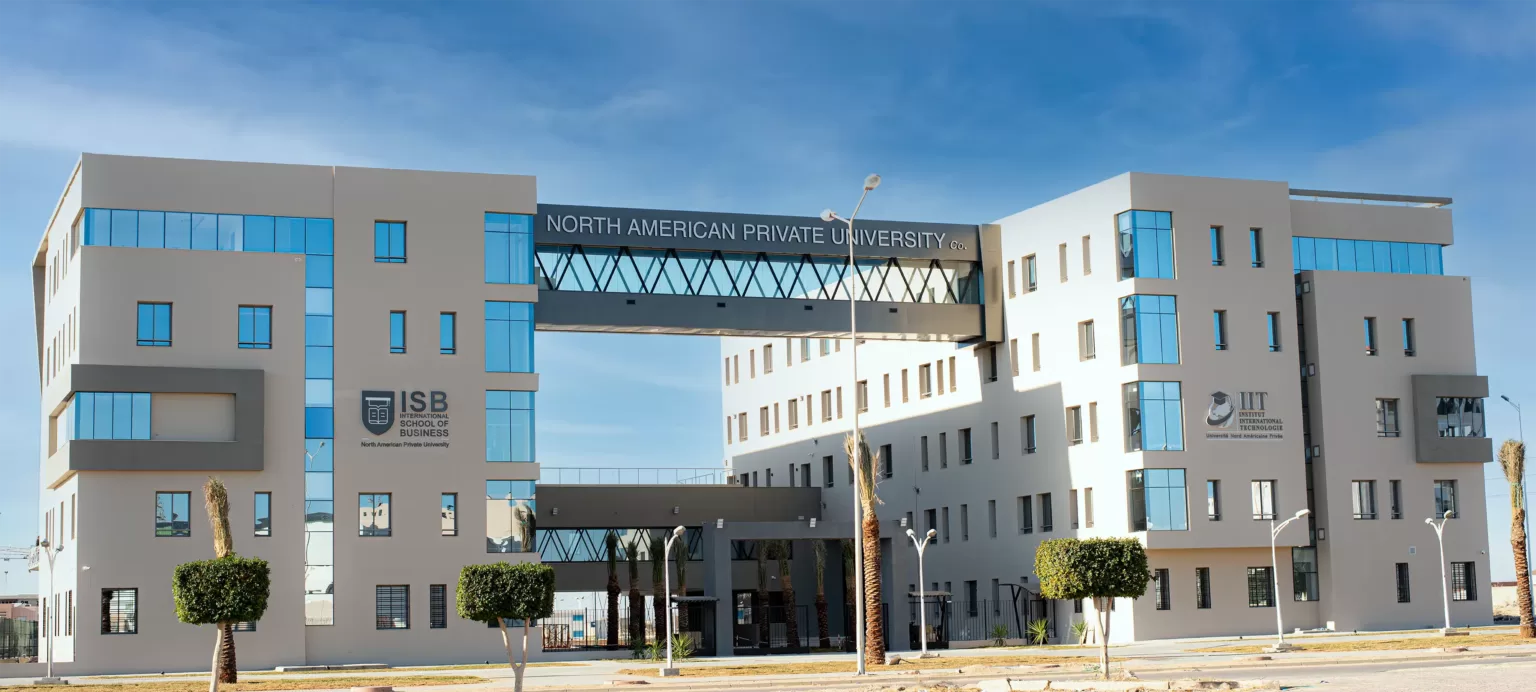
\includegraphics[width=14cm]{images/TemplateImages/Image-Exemple.jpg}}
    \caption{Global use case diagram --- SIPMS platform}
\end{figure}

\begin{table}[H]
\centering
\begin{tabular}{|p{4cm}|p{9cm}|}
\hline
\rowcolor{gray!20}
\textbf{Field} & \textbf{Description} \\
\hline
Use Case & Register a New Candidate \\
\hline
Actor & Receptionist \\
\hline
Precondition & Receptionist is authenticated with RECEPTIONIST role \\
\hline
Main Scenario & 1. Click ``New Candidate'' \newline 2. Fill registration form \newline 3. Upload documents \newline 4. Submit \newline 5. System creates account, generates password, sends email, assigns quiz \\
\hline
Postcondition & Account created; email sent; quiz assigned \\
\hline
Exception & Duplicate email triggers error message \\
\hline
\end{tabular}
\caption{Use case: Register a new candidate}
\end{table}

\begin{table}[H]
\centering
\begin{tabular}{|p{4cm}|p{9cm}|}
\hline
\rowcolor{gray!20}
\textbf{Field} & \textbf{Description} \\
\hline
Use Case & Take a Quiz \\
\hline
Actor & Candidate \\
\hline
Precondition & Candidate is authenticated and a quiz has been assigned \\
\hline
Main Scenario & 1. Navigate to Quiz page \newline 2. Start quiz with timer \newline 3. Answer MCQ questions \newline 4. Submit before timer expires \newline 5. Score is calculated and status updated \\
\hline
Postcondition & Score recorded; status updated \\
\hline
Exception & Timer expiry triggers automatic submission \\
\hline
\end{tabular}
\caption{Use case: Take a quiz}
\end{table}

\section{CONCLUSION}
This chapter provided a complete specification of the SIPMS platform requirements. The actor identification, structured requirements, and use case models serve as the design foundation addressed in the next chapter.


    % Chapter 3 — System Design
    \chapter{SYSTEM DESIGN}
\begin{spacing}{1.2}
\minitoc
\thispagestyle{MyStyle}
\end{spacing}
\newpage

\section{INTRODUCTION}
This chapter presents the technical design of the SIPMS platform. We detail the overall system architecture, the class model with all entities and their relationships, the sequence diagrams for key workflows, and the relational database schema.

\section{GENERAL ARCHITECTURE}

\subsection{Architectural Pattern}
SIPMS follows a \textbf{client-server architecture} with a clear separation of concerns across three tiers:

\begin{itemize}[leftmargin=2cm, topsep=0pt]
    \begin{spacing}{1.25}
        \item \textbf{Presentation Layer}: A React (Vite) single-page application running in the browser, communicating with the backend exclusively via RESTful HTTP requests.
        \item \textbf{Business Logic Layer}: A Spring Boot application exposing a secured REST API, organized into Controllers, Services, and Repositories following the layered architecture pattern.
        \item \textbf{Data Layer}: A MySQL 8 relational database accessed via Spring Data JPA (Hibernate), with schema managed through entity definitions.
    \end{spacing}
\end{itemize}

\begin{figure}[H]
    \centering
    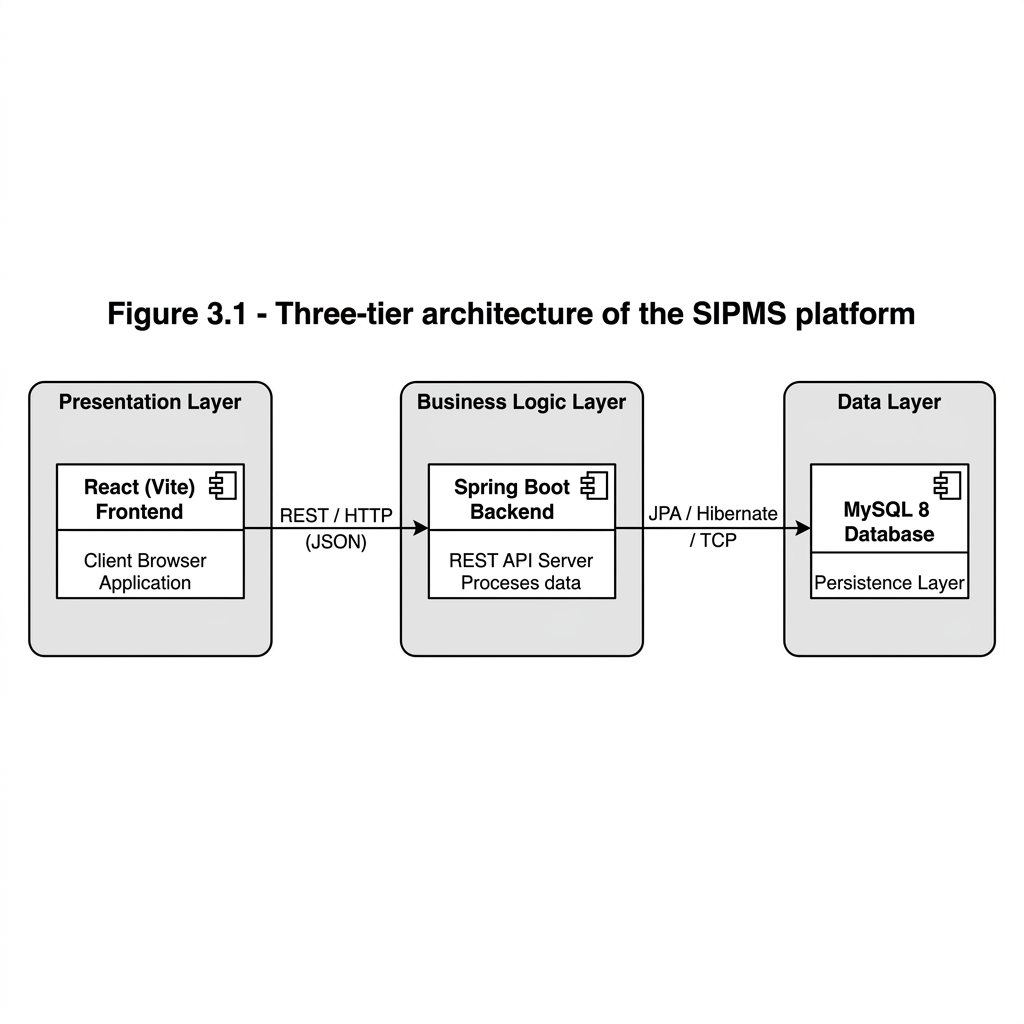
\includegraphics[width=\textwidth]{images/TemplateImages/three_tier_architecture.png}
    \caption{Three-tier architecture of the SIPMS platform}
    \label{fig:three-tier}
\end{figure}

\subsection{Backend Package Structure}
The Spring Boot backend is organized into the following packages:

\begin{table}[H]
\centering
\begin{tabular}{|p{4.5cm}|p{8.5cm}|}
\hline
\rowcolor{gray!20}
\textbf{Package} & \textbf{Responsibility} \\
\hline
\texttt{controller} & Exposes REST endpoints; handles HTTP requests and responses \\
\hline
\texttt{service} & Contains business logic; orchestrates between controllers and repositories \\
\hline
\texttt{repository} & Spring Data JPA interfaces for database access \\
\hline
\texttt{entity} & JPA entity classes mapped to database tables \\
\hline
\texttt{dto} & Data Transfer Objects for request/response payloads \\
\hline
\texttt{security} & JWT filter, authentication entry point, Spring Security configuration \\
\hline
\texttt{common} & Shared utilities: ApiResponse wrapper, FileStorageService, AuditService \\
\hline
\texttt{ai} & AI scoring and matching engine \\
\hline
\end{tabular}
\caption{Backend package structure}
\end{table}

\subsection{Security Architecture}
Authentication in SIPMS is stateless and JWT-based. The security flow operates as follows:

\begin{enumerate}
    \item The client sends credentials (email + password) to \texttt{POST /api/auth/login}.
    \item Spring Security validates credentials via \texttt{UserDetailsService} and BCrypt.
    \item On success, a signed JWT token (HS512) is generated and returned to the client.
    \item For subsequent requests, the client includes the token in the \texttt{Authorization: Bearer} header.
    \item The \texttt{JwtAuthenticationFilter} intercepts every request, validates the token signature and expiration, and populates the \texttt{SecurityContext}.
    \item \texttt{@PreAuthorize} annotations on controller methods enforce role-based access.
\end{enumerate}

\section{CLASS DIAGRAM}

\subsection{Core Entity Relationships}
The domain model consists of 16 entities organised into three subsystems: Core Domain, Quiz Subsystem, and AI Subsystem. The class diagram is decomposed into subsystems to enhance readability and maintain modularity. Each entity corresponds directly to a database table and is involved in at least one use case scenario defined in Chapter 2.

\subsubsection{Core Domain Subsystem}
The core domain subsystem includes the primary business entities that handle authentication, candidate management, applications, and supervision:

\begin{table}[H]
\centering
\small
\begin{tabular}{|p{2.5cm}|p{4cm}|p{6.5cm}|}
\hline
\rowcolor{gray!20}
\textbf{Entity} & \textbf{Key Attributes} & \textbf{Relationships} \\
\hline
\textbf{User} & id, firstName, lastName, email, passwordHash, phone, cin, avatarUrl, active, mustChangePassword, specialty, internshipYear, status, quizScore, createdAt, updatedAt & ManyToMany $\rightarrow$ Role; OneToOne $\leftarrow$ Candidate (optional); OneToMany $\rightarrow$ Notification; OneToMany $\rightarrow$ AuditLog; OneToMany $\rightarrow$ Document (uploadedBy) \\
\hline
\textbf{Role} & id, name (ADMIN, MANAGER, RECEPTIONIST, CANDIDATE) & ManyToMany $\leftarrow$ User \\
\hline
\textbf{Candidate} & id, firstName, lastName, email, phone, cin, assignedQuizId, createdAt, updatedAt & OneToOne $\rightarrow$ User (optional); OneToMany $\rightarrow$ InternshipFile (EAGER); OneToMany $\rightarrow$ Application; OneToMany $\rightarrow$ QuizAttempt; OneToMany $\rightarrow$ Interview \\
\hline
\textbf{InternshipFile} & id, year, university, degree, skillsTags, createdAt, updatedAt & ManyToOne $\rightarrow$ Candidate; OneToMany $\rightarrow$ Document \\
\hline
\textbf{Document} & id, fileName, filePath, fileType, fileSize, documentType (CV, COVER\_LETTER, TRANSCRIPT, ID\_CARD, PHOTO, OTHER), createdAt & ManyToOne $\rightarrow$ Application (optional); ManyToOne $\rightarrow$ InternshipFile (optional); ManyToOne $\rightarrow$ User (uploadedBy) \\
\hline
\textbf{Application} & id, intakeMethod (ONLINE, PHYSICAL), status (8-state DFA), managerNotes, aiMatchScore, decisionDate, createdAt, updatedAt & ManyToOne $\rightarrow$ Candidate (EAGER); ManyToOne $\rightarrow$ Project; ManyToOne $\rightarrow$ Supervisor; ManyToOne $\rightarrow$ User (registeredBy) \\
\hline
\textbf{Supervisor} & id, fullName, email, department, expertiseTags, maxInterns (default 3), currentInterns, bio, active, createdAt & OneToOne $\rightarrow$ User; OneToMany $\rightarrow$ Project; OneToMany $\rightarrow$ Application \\
\hline
\textbf{Project} & id, title, description, domain, technologyTags, requiredSkills, aiScore, status (DRAFT, SUBMITTED, APPROVED, REJECTED), createdAt, updatedAt & ManyToOne $\rightarrow$ User (submittedBy); ManyToOne $\rightarrow$ Supervisor \\
\hline
\textbf{Interview} & id, scheduledAt, interviewer, type (TECHNICAL/HR), status (SCHEDULED/COMPLETED/CANCELLED), score, notes, feedback, createdAt, updatedAt & ManyToOne $\rightarrow$ Candidate; ManyToOne $\rightarrow$ Application \\
\hline
\textbf{Notification} & id, title, message, type (INFO/SUCCESS/WARNING/ERROR), isRead, link, createdAt & ManyToOne $\rightarrow$ User \\
\hline
\textbf{AuditLog} & id, action, entityType, entityId, details, ipAddress, createdAt & ManyToOne $\rightarrow$ User \\
\hline
\end{tabular}
\caption{Core domain subsystem entities}
\end{table}

\subsubsection{Quiz Subsystem}
The quiz subsystem manages assessment creation, question banks, and candidate attempt tracking:

\begin{table}[H]
\centering
\small
\begin{tabular}{|p{2.5cm}|p{4cm}|p{6.5cm}|}
\hline
\rowcolor{gray!20}
\textbf{Entity} & \textbf{Key Attributes} & \textbf{Relationships} \\
\hline
\textbf{Quiz} & id, title, description, durationMins (default 30), passingScore (default 60), totalMarks (default 100), specialty, active, createdAt & ManyToOne $\rightarrow$ User (createdBy); OneToMany $\rightarrow$ QuizQuestion; OneToMany $\rightarrow$ QuizAttempt \\
\hline
\textbf{QuizQuestion} & id, questionText, optionA, optionB, optionC, optionD, correctOption (A/B/C/D), marks (default 5), orderIndex & ManyToOne $\rightarrow$ Quiz \\
\hline
\textbf{QuizAttempt} & id, score, totalMarks, percentage, passed, startedAt, completedAt & ManyToOne $\rightarrow$ Quiz; ManyToOne $\rightarrow$ Candidate; ManyToOne $\rightarrow$ Application; OneToMany $\rightarrow$ QuizAnswer \\
\hline
\end{tabular}
\caption{Quiz subsystem entities}
\end{table}

\subsubsection{AI Subsystem}
The AI subsystem stores the outputs of intelligent ranking and matching operations:

\begin{table}[H]
\centering
\small
\begin{tabular}{|p{2.5cm}|p{4cm}|p{6.5cm}|}
\hline
\rowcolor{gray!20}
\textbf{Entity} & \textbf{Key Attributes} & \textbf{Relationships} \\
\hline
\textbf{AiRanking} & id, rankingType (PROJECT\_RANK, CANDIDATE\_MATCH), referenceId, score (0.0--1.0), reasoning (AI explanation text), createdAt & ManyToOne $\rightarrow$ Supervisor (optional); ManyToOne $\rightarrow$ User (rankedBy) \\
\hline
\end{tabular}
\caption{AI subsystem entities}
\end{table}

\subsection{Relationship Diagram}
The key relationships between entities are summarized as follows:

\begin{verbatim}
User *-- Role (ManyToMany)
Candidate "1" --> "0..1" User (optional OneToOne)
Candidate "1" *--> "0..*" InternshipFile (OneToMany, EAGER)
InternshipFile "1" *--> "0..*" Document (OneToMany)
Application "1" --> "0..*" Document (OneToMany)
Candidate "1" *--> "0..*" Application (OneToMany)
Application "1" --> "0..1" Project (ManyToOne)
Application "1" --> "0..1" Supervisor (ManyToOne)
Application "1" --> "0..1" User (registeredBy)
Supervisor "1" *--> "0..*" Project (OneToMany)
Supervisor "1" --> "0..1" User (OneToOne)
Quiz "1" *--> "0..*" QuizQuestion (OneToMany)
Quiz "1" *--> "0..*" QuizAttempt (OneToMany)
Candidate "1" *--> "0..*" QuizAttempt (OneToMany)
Application "1" *--> "0..*" QuizAttempt (OneToMany)
Candidate "1" *--> "0..*" Interview (OneToMany)
Application "1" *--> "0..*" Interview (OneToMany)
User "1" *--> "0..*" Quiz (createdBy)
User "1" *--> "0..*" Notification (OneToMany)
User "1" *--> "0..*" AuditLog (OneToMany)
Supervisor "1" --> "0..*" AiRanking (OneToMany)
User "1" --> "0..*" AiRanking (rankedBy)
\end{verbatim}

Beyond data-level entity relationships, the system also defines the following \texttt{<<include>>} and \texttt{<<extend>>} relationships between use cases, capturing functional dependencies and optional extensions:

\begin{verbatim}
--- Include Relationships (mandatory) ---
Login                  <<include>>   Complete Assigned Quiz
Login                  <<include>>   Register Candidate
Login                  <<include>>   Upload CV for AI Analysis
Complete Assigned Quiz <<include>>   Generate AI Ranking
Complete Assigned Quiz <<include>>   Schedule Interview
Generate AI Ranking    <<include>>   Assign Supervisor to Candidate

--- Extend Relationships (optional) ---
Register Candidate     <<extend>>    Upload CV for AI Analysis
Complete Assigned Quiz <<extend>>    Send Automated Email Notification
Update Application     <<extend>>    Send Automated Email Notification
Schedule Interview     <<extend>>    Send Automated Email Notification
\end{verbatim}

\begin{figure}[H]
    \centering
    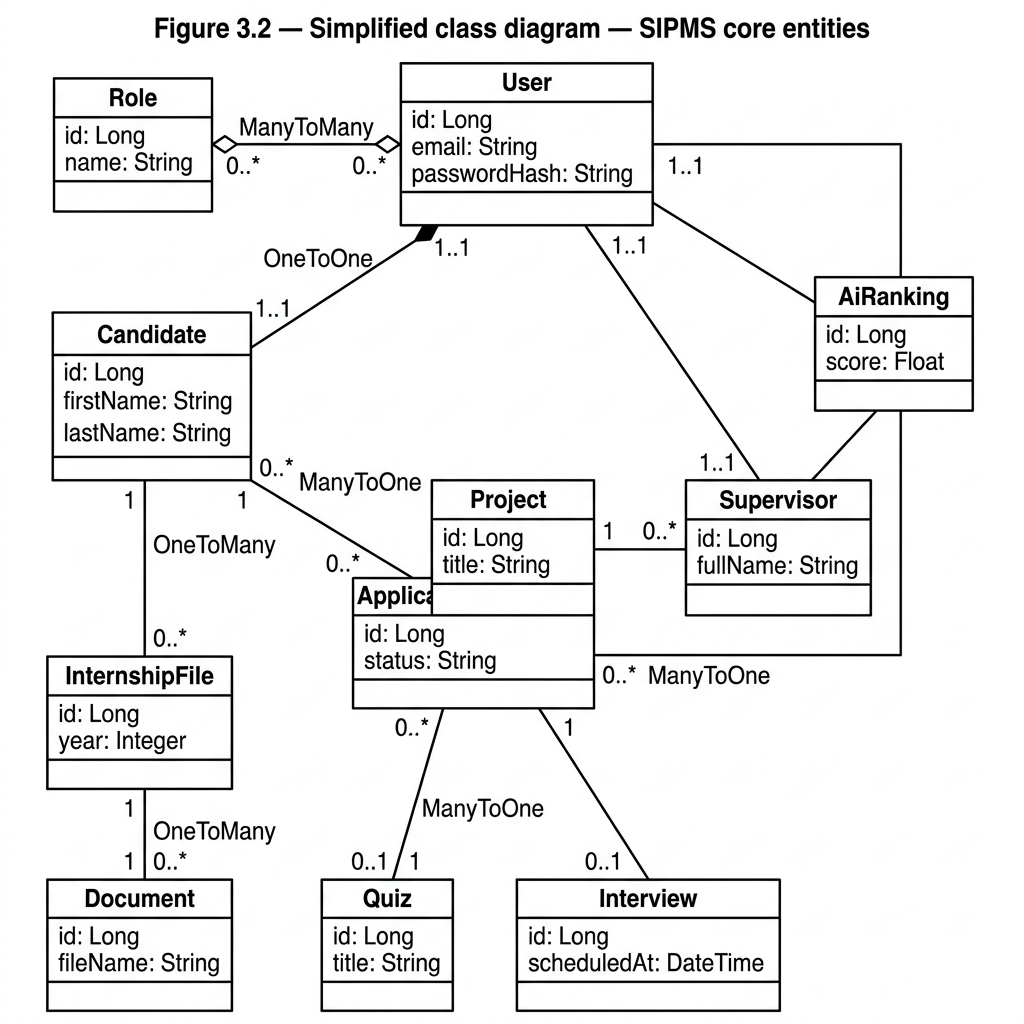
\includegraphics[width=\textwidth]{images/TemplateImages/simplified_class_diagram.png}
    \caption{Simplified class diagram --- SIPMS core entities}
    \label{fig:class-diagram}
\end{figure}

\subsection{Entity Interaction and Call Flow}
The class diagram defines the static structure, but the dynamic behavior is governed by how these entities call one another during runtime. The key interaction flows are as follows:

\renewcommand{\labelitemi}{\tiny$\bullet$}
\begin{itemize}[leftmargin=2cm, topsep=4pt]
    \begin{spacing}{1.25}
        \item \textbf{Authentication flow}: \texttt{User} $\rightarrow$ \texttt{Role} (via ManyToMany). The \texttt{JwtAuthenticationFilter} reads the authenticated \texttt{User}'s roles from the \texttt{SecurityContext} and enforces access via \texttt{@PreAuthorize} annotations on controller methods.
        \item \textbf{Candidate registration flow}: \texttt{Frontend} $\rightarrow$ \texttt{CandidateController} $\rightarrow$ \texttt{CandidateService} $\rightarrow$ \texttt{CandidateRepository} saves a new \texttt{Candidate}. The optional \texttt{User} entity is NOT created at this stage — it is created later during the manager approval step (\texttt{approveAndSendQuiz()}), which establishes the OneToOne link from \texttt{Candidate} to \texttt{User}.
        \item \textbf{Internship file upload flow}: \texttt{Frontend} $\rightarrow$ \texttt{CandidateController} $\rightarrow$ \texttt{CandidateService} $\rightarrow$ \texttt{InternshipFileRepository} saves the \texttt{InternshipFile} linked to the \texttt{Candidate}. If a document is attached, \texttt{FileStorageService} writes the file to disk, then a \texttt{Document} entity is created and added to the \texttt{InternshipFile}'s documents collection.
        \item \textbf{Quiz assignment and evaluation flow}: \texttt{Manager} approves candidate $\rightarrow$ \texttt{CandidateService.approveAndSendQuiz()} $\rightarrow$ creates \texttt{User} (optional OneToOne), reads or creates \texttt{Quiz}, creates \texttt{QuizAttempt} linking \texttt{Candidate}, \texttt{Quiz}, and \texttt{Application}. When the candidate submits answers, \texttt{QuizService} grades them, persists \texttt{QuizAnswer} records, updates \texttt{QuizAttempt.score/percentage/passed}, and advances the \texttt{Application.status}.
        \item \textbf{Interview scheduling flow}: \texttt{Manager} $\rightarrow$ \texttt{InterviewController} $\rightarrow$ \texttt{InterviewService} $\rightarrow$ saves \texttt{Interview} with references to \texttt{Candidate} and \texttt{Application}. When the result is recorded, \texttt{Interview.score}, \texttt{Interview.notes}, and \texttt{Interview.feedback} are updated, and the \texttt{Interview.status} transitions from \texttt{SCHEDULED} to \texttt{COMPLETED}.
        \item \textbf{AI evaluation flow}: \texttt{Manager} triggers AI matching $\rightarrow$ \texttt{AiService} $\rightarrow$ reads \texttt{Candidate}'s skills (via \texttt{InternshipFile.skillsTags}), quiz performance (\texttt{QuizAttempt.percentage}), and project requirements (\texttt{Project.domain}, \texttt{Project.technologyTags}). The weighted score is computed and persisted as an \texttt{AiRanking} record linked to the \texttt{Supervisor}. The \texttt{Application.aiMatchScore} field is also updated for quick reference on the manager dashboard.
    \end{spacing}
\end{itemize}

\subsection{AI Entities and Scoring Logic}
The AI module introduces two specialized concepts that are embedded across multiple entities:

\subsubsection{AI Scoring Fields}
AI-generated scores are stored directly on existing entities to avoid joins and simplify queries:

\begin{itemize}[leftmargin=2cm, topsep=4pt]
    \begin{spacing}{1.25}
        \item \textbf{Application.aiMatchScore} (Double): A value between 0.0 and 1.0 representing the AI's confidence that the candidate is a good fit for the assigned project. Calculated by analyzing the candidate's quiz score (\texttt{QuizAttempt.percentage}), skills tags (\texttt{InternshipFile.skillsTags}), and degree level against the project's domain and technology requirements.
        \item \textbf{Project.aiScore} (Double): A value between 0.0 and 1.0 representing the overall quality and relevance score of a project proposal. Calculated based on description completeness, domain alignment with company priorities, and the submitting candidate's profile strength.
    \end{spacing}
\end{itemize}

\subsubsection{AiRanking Entity}
The \texttt{AiRanking} entity stores the output of AI-based ranking operations:

\begin{itemize}[leftmargin=2cm, topsep=4pt]
    \begin{spacing}{1.25}
        \item \textbf{rankingType}: An enum with two values — \texttt{PROJECT\_RANK} (ranks projects by relevance for a given candidate) and \texttt{CANDIDATE\_MATCH} (ranks candidates by suitability for a given supervisor).
        \item \textbf{referenceId}: The ID of the ranked entity (project ID for PROJECT\_RANK, candidate ID for CANDIDATE\_MATCH).
        \item \textbf{score}: A Double between 0.0 and 1.0 representing the AI's confidence score.
        \item \textbf{reasoning}: A free-text field containing the AI's natural language explanation of the score. Example: \textit{"Candidate has strong Java and Spring Boot skills matching the supervisor's expertise. Quiz score of 85\% indicates solid technical foundation."}
        \item \textbf{supervisor}: Optional ManyToOne to Supervisor. Present only when the ranking is a CANDIDATE\_MATCH targeting a specific supervisor.
        \item \textbf{rankedBy}: The User (Admin/Manager) who triggered the AI evaluation.
    \end{spacing}
\end{itemize}

\subsubsection{AI Scoring Algorithm}
The AI scoring follows a weighted formula:

\begin{verbatim}
AI Match Score = w1 x skillOverlap + w2 x quizPerformance + w3 x academicLevel

Where:
  skillOverlap    = |candidateSkills and projectSkills| / |projectSkills|
  quizPerformance = QuizAttempt.percentage / 100
  academicLevel   = degreeLevel / maxDegreeLevel

Default weights: w1=0.40, w2=0.40, w3=0.20
\end{verbatim}

These scores are computed by the \texttt{AiService} which delegates to the configured AI provider (GPT-4-mini) for the reasoning generation, while the numerical scoring uses deterministic formulas for consistency and reproducibility.

\section{SEQUENCE DIAGRAMS}

Five sequence diagrams are presented in this section to illustrate the dynamic behaviour of the SIPMS platform. Each diagram corresponds to one or more use cases defined in Chapter 2 and models the interactions between actors, frontend components, backend services, and the database.

\subsection{Sequence: Candidate Registration with Internship File Upload}
This sequence describes the complete candidate registration and document upload flow performed by the receptionist. It corresponds to the use cases \textbf{Register a New Candidate} and \textbf{Add Internship File with Document}.

\begin{enumerate}
    \item The receptionist fills the candidate form (firstName, lastName, email, phone, CIN) and submits it via the React frontend.
    \item The frontend calls \texttt{POST /api/candidates} with the candidate data as a JSON payload.
    \item \texttt{CandidateService.createCandidate()} validates the input, persists the \texttt{Candidate} entity to the database, and returns the created record with its generated identifier.
    \item The receptionist then opens the internship file form and enters the year, university, degree, and skills tags. Optionally, a PDF document may be attached.
    \item The frontend calls \texttt{POST /api/candidates/\{id\}/internship-files/with-document} using multipart form data to transmit both the metadata and the uploaded file.
    \item \texttt{FileStorageService.storeFile()} saves the uploaded document to \texttt{./uploads/candidates/\{id\}/} with a UUID-based filename to prevent path traversal and naming collisions.
    \item An \texttt{InternshipFile} entity is persisted and linked to the candidate. If a file was uploaded, a \texttt{Document} entity is also persisted and associated with the \texttt{InternshipFile}.
    \item The frontend refreshes the candidates table and the internship files list to reflect the newly added data.
\end{enumerate}

\begin{figure}[H]
    \centering
    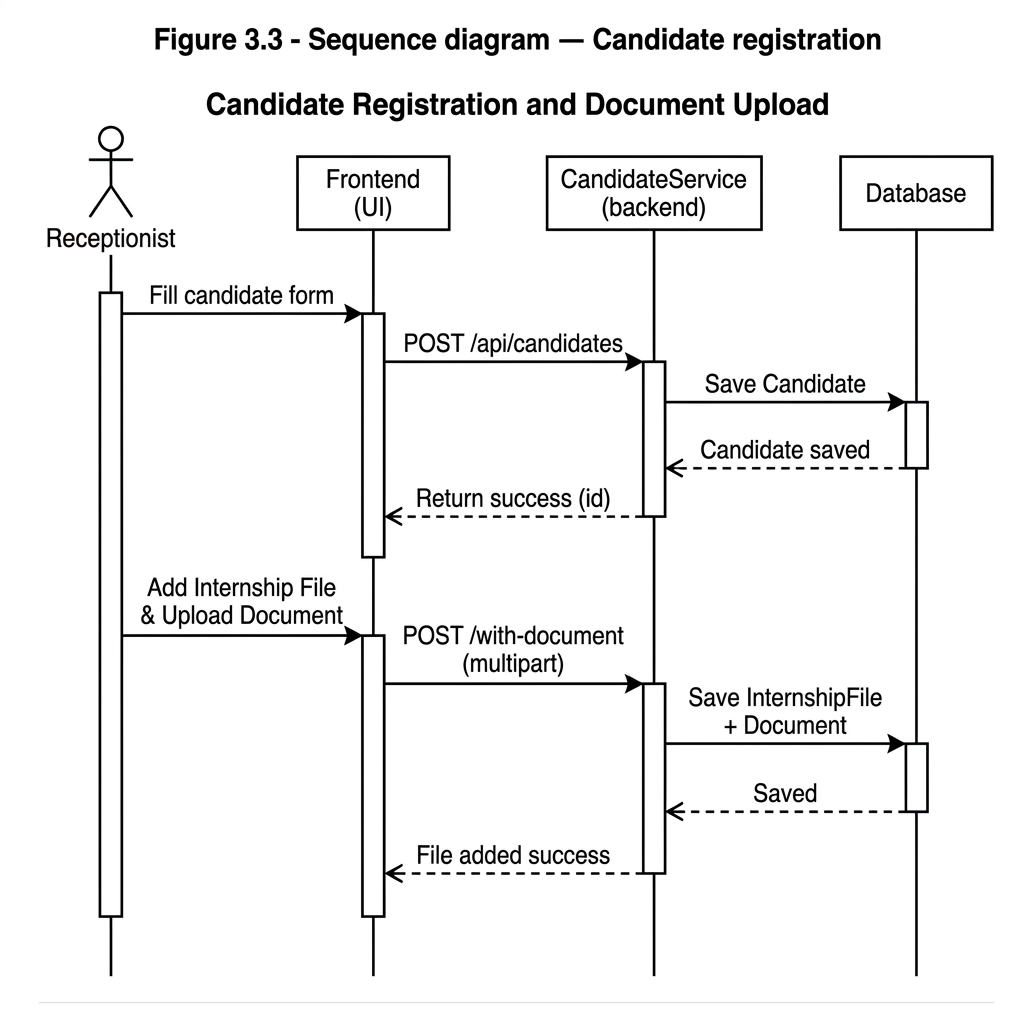
\includegraphics[width=\textwidth]{images/TemplateImages/sequence_candidate_registration.png}
    \caption{Sequence diagram --- Candidate registration with document upload}
    \label{fig:sequence-registration}
\end{figure}

\subsection{Sequence: Approve Candidate and Send Quiz}
This sequence corresponds to the use case \textbf{Approve and Send Quiz} (User Story US-18) and models the manager's approval workflow.

\begin{enumerate}
    \item The manager selects a candidate from the candidates table and clicks "Approve \& Send Quiz".
    \item The \texttt{QuizSelectionModal} opens and loads existing quizzes via \texttt{GET /api/quizzes} for the manager to choose from.
    \item The manager either selects an existing quiz from the list or opts to create a default 5-question MCQ quiz.
    \item The frontend calls \texttt{POST /api/candidates/\{id\}/approve-and-send-quiz} with an optional \texttt{quizId} in the request body.
    \item \texttt{CandidateService.approveAndSendQuiz()} performs the following steps transactionally:
        \begin{enumerate}
            \item Creates a \texttt{User} account for the candidate with a BCrypt-hashed temporary password and sets the \texttt{mustChangePassword} flag.
            \item If a \texttt{quizId} was provided, creates a \texttt{QuizAttempt} linking the candidate to the existing quiz.
            \item If no \texttt{quizId} was provided, creates a new \texttt{Quiz} containing 5 default MCQs, then creates the corresponding \texttt{QuizAttempt}.
            \item Sends an HTML email via Gmail SMTP containing the candidate's login credentials and the assigned quiz title.
        \end{enumerate}
    \item The frontend refreshes the candidates view, displaying the candidate with an active user account and an assigned quiz status.
\end{enumerate}

\subsection{Sequence: Interview Scheduling and Result Recording}
This sequence corresponds to the use cases \textbf{Schedule Interview} and \textbf{Record Interview Result} (User Stories US-19 and US-20).

\begin{enumerate}
    \item The manager identifies a candidate whose application is in \texttt{QUIZ\_COMPLETED} status and who has passed the quiz (\texttt{passed = true}).
    \item The manager clicks "Schedule Interview" and fills the scheduling form with a date and time, interviewer name, and interview type (TECHNICAL or HR).
    \item The frontend calls \texttt{POST /api/interviews} with the candidate identifier, application identifier, scheduled timestamp, interviewer, and type.
    \item \texttt{InterviewService.createInterview()} validates the scheduling constraints and persists the interview with status \texttt{SCHEDULED}.
    \item The newly scheduled interview appears in the interview management page alongside existing records.
    \item After the interview takes place, the manager records the result by calling \texttt{PUT /api/interviews/\{id\}/result} with the score, notes, and feedback. The service updates the interview status to \texttt{COMPLETED} and persists the evaluation data.
\end{enumerate}

\section{DATABASE SCHEMA}

\subsection{Main Tables}
\begin{table}[H]
\centering
\small
\begin{tabular}{|p{3cm}|p{10cm}|}
\hline
\rowcolor{gray!20}
\textbf{Table} & \textbf{Key Columns} \\
\hline
\texttt{users} & id, first\_name, last\_name, email, password\_hash, phone, cin, avatar\_url, active, must\_change\_password, specialty, internship\_year, status, quiz\_score, quiz\_created\_at, quiz\_completed\_at, created\_at, updated\_at \\
\hline
\texttt{roles} & id, name (ADMIN, MANAGER, RECEPTIONIST, CANDIDATE) \\
\hline
\texttt{user\_roles} & user\_id, role\_id \\
\hline
\texttt{candidates} & id, first\_name, last\_name, email, phone, cin, assigned\_quiz\_id, user\_id (nullable FK), created\_at, updated\_at \\
\hline
\texttt{internship\_files} & id, candidate\_id (FK), year, university, degree, skills\_tags, created\_at, updated\_at \\
\hline
\texttt{documents} & id, application\_id (nullable FK), internship\_file\_id (nullable FK), uploaded\_by (FK), file\_name, file\_path, file\_type, file\_size, document\_type (CV, COVER\_LETTER, TRANSCRIPT, ID\_CARD, PHOTO, OTHER), created\_at \\
\hline
\texttt{applications} & id, candidate\_id (FK), project\_id (FK), supervisor\_id (FK), registered\_by (FK), intake\_method (ONLINE, PHYSICAL), status (PENDING..REJECTED), manager\_notes, decision\_date, ai\_match\_score, created\_at, updated\_at \\
\hline
\texttt{supervisors} & id, user\_id (FK), full\_name, email, department, expertise\_tags, max\_interns, current\_interns, bio, active, created\_at \\
\hline
\texttt{projects} & id, title, description, domain, technology\_tags, required\_skills, status (DRAFT, SUBMITTED, APPROVED, REJECTED), ai\_score, submitted\_by (FK), supervisor\_id (FK), created\_at, updated\_at \\
\hline
\texttt{quizzes} & id, title, description, duration\_mins, passing\_score, total\_marks, specialty, active, created\_by (FK), created\_at \\
\hline
\texttt{quiz\_questions} & id, quiz\_id (FK), question\_text, option\_a, option\_b, option\_c, option\_d, correct\_option, marks, order\_index \\
\hline
\texttt{quiz\_attempts} & id, quiz\_id (FK), candidate\_id (FK), application\_id (FK), score, total\_marks, percentage, passed, started\_at, completed\_at \\
\hline
\texttt{quiz\_answers} & id, attempt\_id (FK), question\_id (FK), selected\_option, is\_correct \\
\hline
\texttt{interviews} & id, candidate\_id (FK), application\_id (FK), scheduled\_at, interviewer, type (TECHNICAL, HR), status (SCHEDULED, COMPLETED, CANCELLED), score, notes, feedback, created\_at, updated\_at \\
\hline
\texttt{notifications} & id, user\_id (FK), title, message, type (INFO, SUCCESS, WARNING, ERROR), is\_read, link, created\_at \\
\hline
\texttt{audit\_log} & id, user\_id (FK), action, entity\_type, entity\_id, details, ip\_address, created\_at \\
\hline
\texttt{ai\_rankings} & id, ranking\_type (PROJECT\_RANK, CANDIDATE\_MATCH), reference\_id, score, reasoning, supervisor\_id (FK), ranked\_by (FK), created\_at \\
\hline
\end{tabular}
\caption{Complete database schema (17 tables)}
\end{table}

\subsection{Normalization Analysis}
The database schema is designed to comply with \textbf{Third Normal Form (3NF)} to minimize data redundancy and ensure referential integrity:

\begin{itemize}[leftmargin=2cm, topsep=4pt]
    \begin{spacing}{1.25}
        \item \textbf{First Normal Form (1NF)}: All tables have a single-column primary key (\texttt{id}) with auto-increment. Every column contains atomic values — for example, \texttt{skills\_tags} stores comma-separated tags as a single string (denormalized for simplicity), while multi-valued attributes like quiz options use separate columns (\texttt{option\_a}, \texttt{option\_b}, etc.) rather than arrays or JSON.
        \item \textbf{Second Normal Form (2NF)}: All non-key columns are fully functionally dependent on the primary key. There are no partial dependencies because every table uses a single-column primary key. For example, \texttt{documents.file\_name} depends only on \texttt{documents.id}, not on any candidate or application attribute.
        \item \textbf{Third Normal Form (3NF)}: No transitive dependencies exist. Every non-key column depends directly on the primary key, not on another non-key column. For instance, \texttt{quizzes.passing\_score} depends only on \texttt{quizzes.id}, not on \texttt{quizzes.specialty} or \texttt{quizzes.title}.
    \end{spacing}
\end{itemize}

Small controlled denormalizations were intentionally applied for performance:
\begin{itemize}[leftmargin=2cm, topsep=4pt]
    \begin{spacing}{1.25}
        \item \textbf{Application.aiMatchScore} and \textbf{Project.aiScore} are stored directly on the entity rather than in a separate scores table, avoiding a join on every dashboard load.
        \item \textbf{InternshipFile.skillsTags} uses a comma-separated string rather than a junction table, since tags are small in number and always retrieved together with the file record.
    \end{spacing}
\end{itemize}

\subsection{Constraints and Integrity Rules}
The schema enforces the following constraints to guarantee data quality:

\begin{itemize}[leftmargin=2cm, topsep=4pt]
    \begin{spacing}{1.25}
        \item \textbf{NOT NULL constraints} on all business-critical columns: \texttt{users.email}, \texttt{candidates.email}, \texttt{internship\_files.year}, \texttt{applications.status}, \texttt{interviews.scheduled\_at}, \texttt{documents.file\_name}.
        \item \textbf{UNIQUE constraints}: \texttt{users.email} is unique to prevent duplicate accounts. \texttt{candidates.email} is also unique to prevent duplicate registrations.
        \item \textbf{CHECK constraints} enforced via Java enums mapped to MySQL ENUM columns: \texttt{applications.status} (PENDING, UNDER\_REVIEW, QUIZ\_PENDING, QUIZ\_COMPLETED, AI\_EVALUATING, MANAGER\_REVIEW, ACCEPTED, REJECTED), \texttt{interviews.type} (TECHNICAL, HR), \texttt{documents.document\_type} (CV, COVER\_LETTER, TRANSCRIPT, ID\_CARD, PHOTO, OTHER).
        \item \textbf{DEFAULT values}: \texttt{applications.status} defaults to \texttt{PENDING}, \texttt{interviews.status} defaults to \texttt{SCHEDULED}, \texttt{quizzes.active} defaults to \texttt{true}.
        \item \textbf{CASCADE rules}: Deleting a \texttt{Candidate} cascades to all linked \texttt{InternshipFile} and \texttt{Application} records. Deleting an \texttt{InternshipFile} cascades to its \texttt{Document} records.
        \item \textbf{Foreign key constraints}: Every \texttt{FOREIGN KEY} ensures that referenced records exist. For example, \texttt{internship\_files.candidate\_id} references \texttt{candidates.id} and prevents orphaned records.
    \end{spacing}
\end{itemize}

\subsection{Schema Design Decisions}
The relational schema follows the entity relationships described in Section 3.3. Foreign key constraints enforce referential integrity across all tables. Key design decisions include:

\begin{itemize}[leftmargin=2cm, topsep=0pt]
    \begin{spacing}{1.25}
        \item \textbf{Nullable foreign keys}: \texttt{documents.application\_id} and \texttt{documents.internship\_file\_id} are both nullable because a document can belong to either an application or an internship file, but not necessarily both.
        \item \textbf{Optional User link}: \texttt{candidates.user\_id} is nullable because a candidate exists independently of a User account. The User is created only when the manager invites/approves the candidate.
        \item \textbf{Enum types}: Status fields (application status, interview status, document type) are stored as MySQL ENUM types for data integrity.
        \item \textbf{Audit timestamps}: All entities include \texttt{created\_at} and most include \texttt{updated\_at}, populated automatically via JPA's \texttt{@PrePersist} and \texttt{@PreUpdate} hooks.
    \end{spacing}
\end{itemize}

\subsection{Diagram Quality and Formal Coherence}
The UML diagrams presented in this chapter adhere to standard modeling conventions and maintain formal coherence across all levels of abstraction. The following quality criteria were applied:

\renewcommand{\labelitemi}{\tiny$\bullet$}
\begin{itemize}[leftmargin=2cm, topsep=4pt]
    \begin{spacing}{1.25}
        \item \textbf{UML compliance}: Class diagrams follow UML 2.5 notation with correct multiplicity markers (\texttt{1}, \texttt{0..*}, \texttt{0..1}), directed associations for foreign key relationships, and diamond-free aggregation since all relationships are standard associations with explicit JPA annotations. Associations are annotated with fetch types (EAGER vs LAZY) and cascade behaviors where relevant.
        \item \textbf{Cross-diagram traceability}: Every entity in the class diagram participates in at least one sequence diagram interaction. For example, the \texttt{Candidate} entity appears in the registration sequence, the quiz sequence, and the interview sequence. Each sequence diagram, in turn, corresponds to a specific use case described in Chapter 2, ensuring end-to-end traceability from requirements to design.
        \item \textbf{Subsystem consistency}: The decomposition into Core Domain, Quiz, and AI subsystems in the class diagram aligns with the five functional modules defined in the system decomposition (Chapter 2). Entities within each subsystem have cohesive responsibilities and minimal cross-subsystem dependencies, reducing coupling and improving maintainability.
        \item \textbf{Entity-to-table mapping}: Each class diagram entity maps directly to a MySQL database table via JPA \texttt{@Entity} and \texttt{@Table} annotations. Field-level \texttt{@Column} mappings define column names, nullability, lengths, and constraints, ensuring database schema coherence with the domain model. This one-to-one mapping eliminates impedance mismatch between the object-oriented and relational representations.
        \item \textbf{Behavioral consistency}: Sequence diagrams model the dynamic behavior of the system in a way that is consistent with the static structure defined in the class diagram. Lifelines correspond to controller, service, and entity instances derived from the class model, while messages map to method calls on those instances. The state machine for application lifecycle transitions is consistent with the status field defined on the \texttt{Application} entity, and every valid transition corresponds to a guard condition enforced in the service layer.
        \item \textbf{Normalization and denormalization balance}: The schema achieves 3NF for transactional data while applying controlled denormalizations (\texttt{Application.aiMatchScore}, \texttt{InternshipFile.skillsTags}) for performance-critical read paths, as detailed in Section 3.5.3. This balance ensures data integrity without sacrificing query performance.
    \end{spacing}
\end{itemize}

\section{CONCLUSION}
This chapter presented the complete technical design of SIPMS, covering the three-tier client-server architecture, the JWT-based stateless security model with HS512 signing and BCrypt password hashing, and the full class diagram decomposed into three subsystems (Core Domain with 11 entities, Quiz subsystem with 3 entities, and AI subsystem). The entity-relationship diagram and use case include/extend dependencies were formalised to ensure traceability between the static structure and dynamic behaviour of the system. Five sequence diagrams illustrated the key workflows — authentication, candidate registration, quiz approval and completion, interview scheduling, and CV analysis — each consistent with the use cases defined in Chapter 2. The database schema was presented with 17 tables, normalised to 3NF with controlled denormalisations for performance, and enforced through foreign key, unique, check, and cascade constraints. These design decisions provide a solid blueprint for the implementation phase described in the next chapter.

    
    % Chapter 4 — Implementation
    \chapter{IMPLEMENTATION}
\begin{spacing}{1.2}
\minitoc
\thispagestyle{MyStyle}
\end{spacing}
\newpage

\section{INTRODUCTION}
This chapter presents the practical realization of the SIPMS platform. We first describe the development environment and tools used, then walk through the four Scrum sprints executed during the project, presenting the key user interfaces delivered in each sprint.

\section{DEVELOPMENT ENVIRONMENT}

\subsection{Hardware Environment}
\begin{table}[H]
\centering
\begin{tabular}{|p{4cm}|p{9cm}|}
\hline
\rowcolor{gray!20}
\textbf{Component} & \textbf{Specification} \\
\hline
Processor & Intel Core i5 / i7, 2.4 GHz or higher \\
\hline
RAM & 16 GB \\
\hline
Storage & 512 GB SSD \\
\hline
Operating System & Windows 10 / 11 (64-bit) \\
\hline
\end{tabular}
\caption{Hardware development environment}
\end{table}

\subsection{Software Environment}
\begin{table}[H]
\centering
\begin{tabular}{|p{4cm}|p{4cm}|p{5cm}|}
\hline
\rowcolor{gray!20}
\textbf{Tool / Technology} & \textbf{Version} & \textbf{Purpose} \\
\hline
Java (JDK) & 17 LTS & Backend runtime \\
\hline
Spring Boot & 3.2.x & Backend framework \\
\hline
Maven & 3.9.x & Build and dependency management \\
\hline
MySQL & 8.0 & Relational database \\
\hline
Node.js & 20 LTS & Frontend runtime \\
\hline
React (Vite) & 18 / 5.x & Frontend framework \\
\hline
VS Code & Latest & Frontend IDE \\
\hline
IntelliJ IDEA & 2023.x & Backend IDE \\
\hline
Postman & Latest & API testing \\
\hline
Git / GitHub & - & Version control \\
\hline
MySQL Workbench & 8.0 & Database management \\
\hline
\end{tabular}
\caption{Software development environment}
\end{table}

\section{SPRINT 1 — AUTHENTICATION AND USER MANAGEMENT}

\subsection{Sprint Backlog}
\begin{table}[H]
\centering
\begin{tabular}{|p{1cm}|p{8cm}|p{3cm}|}
\hline
\rowcolor{gray!20}
\textbf{\#} & \textbf{User Story} & \textbf{Status} \\
\hline
1 & As a user, I want to log in with my email and password and receive a JWT token & Done \\
\hline
2 & As a user, I want to be redirected to my role-specific dashboard after login & Done \\
\hline
3 & As a new user, I want to be prompted to change my temporary password on first login & Done \\
\hline
4 & As an admin, I want to create, view, edit, and delete user accounts & Done \\
\hline
5 & As a system, I must enforce RBAC so that each route is accessible only to authorized roles & Done \\
\hline
\end{tabular}
\caption{Sprint 1 backlog}
\end{table}

\subsection{Key Technical Implementations}
\begin{itemize}[leftmargin=2cm, topsep=0pt]
    \begin{spacing}{1.25}
        \item \textbf{JwtTokenProvider}: Generates and validates tokens using a configurable secret key and expiry duration.
        \item \textbf{JwtAuthenticationFilter}: Intercepts all requests, extracts and validates the Bearer token, and populates the Spring Security context.
        \item \textbf{SecurityConfig}: Defines the HTTP security rules, CORS configuration, and public endpoints (\texttt{/api/auth/**}).
        \item \textbf{RoleBasedRedirect}: A React component that reads the user's role from the JWT and redirects to the appropriate dashboard path.
        \item \textbf{ProtectedRoute}: Guards frontend routes by checking authentication state and role membership.
    \end{spacing}
\end{itemize}

\subsection{Delivered Interfaces}

\begin{figure}[H]
    \centering
    \fbox{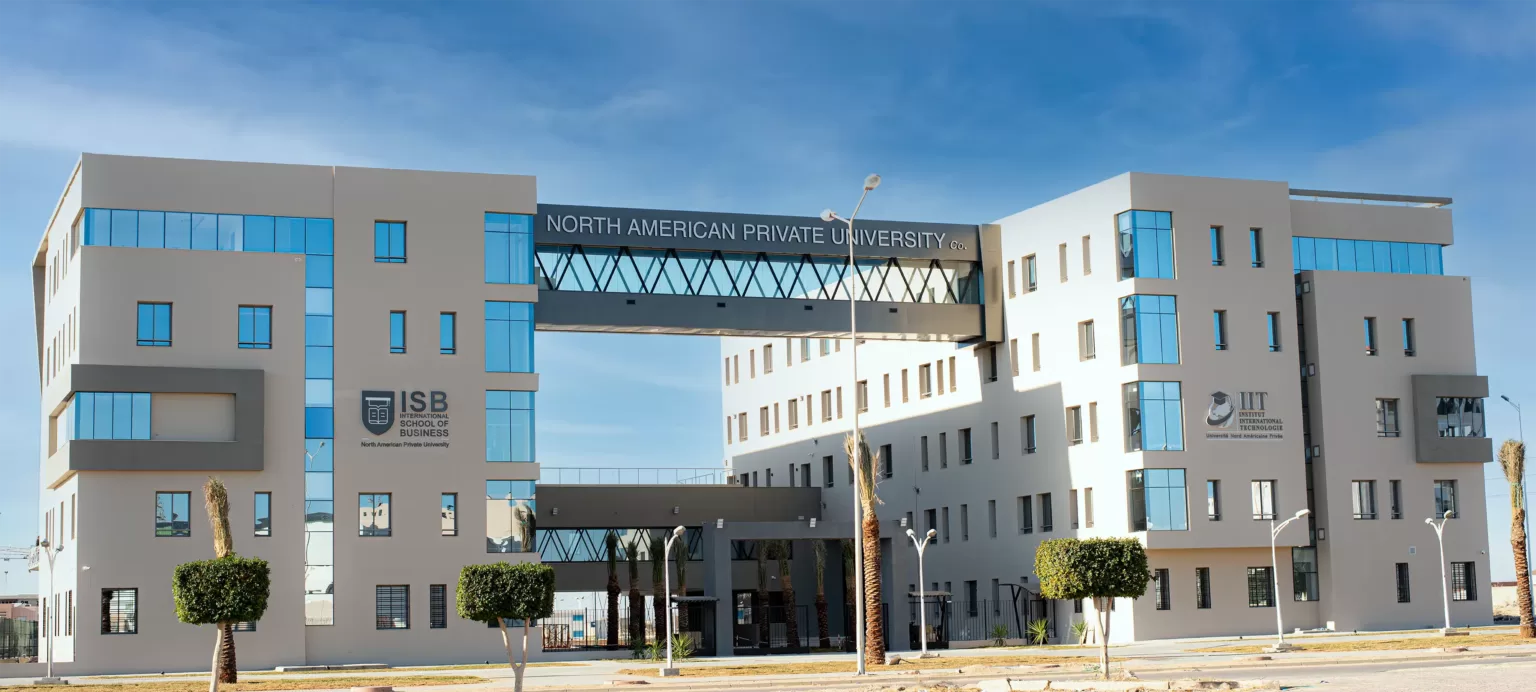
\includegraphics[width=13cm]{images/TemplateImages/Image-Exemple.jpg}}
    \caption{Login page --- SIPMS CLINISYS branding}
\end{figure}

\begin{figure}[H]
    \centering
    \fbox{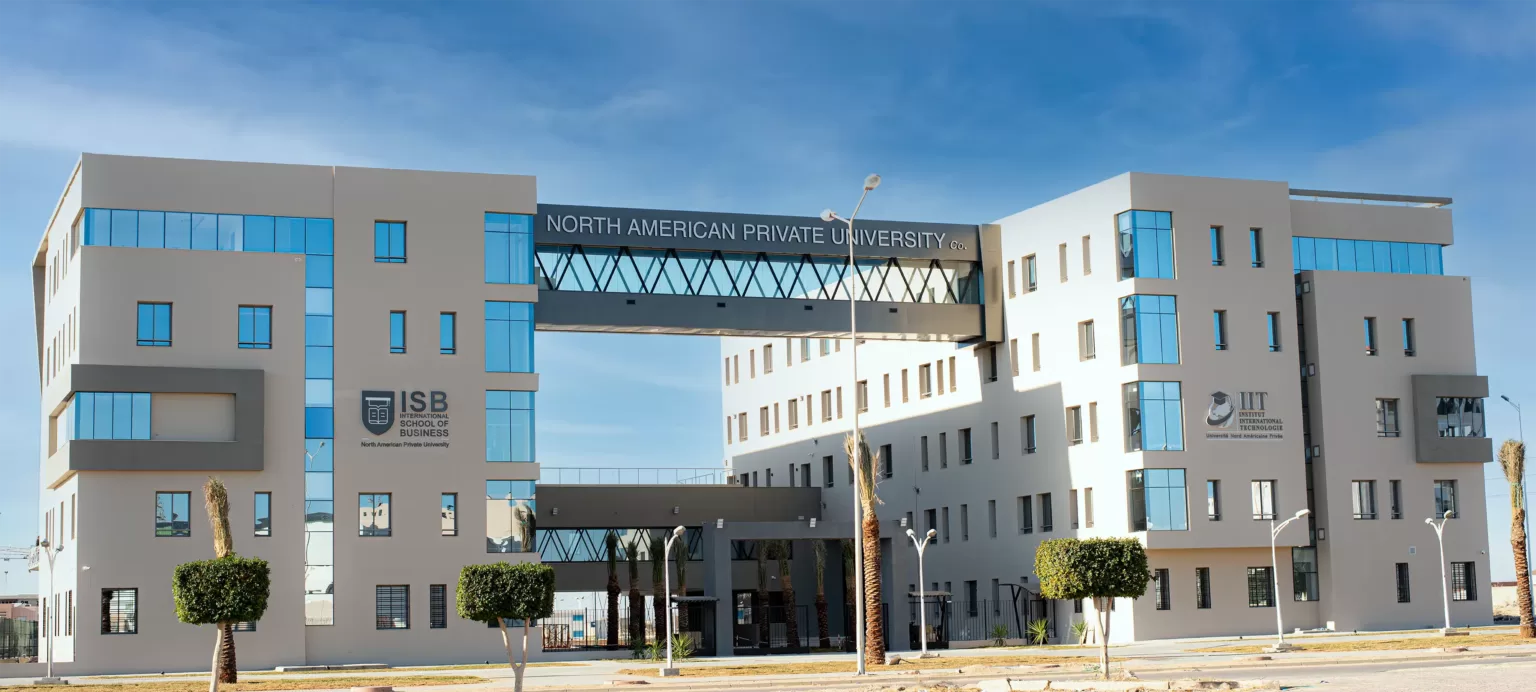
\includegraphics[width=13cm]{images/TemplateImages/Image-Exemple.jpg}}
    \caption{Administrator dashboard --- Users management panel}
\end{figure}

\section{SPRINT 2 — RECEPTION MODULE}

\subsection{Sprint Backlog}
\begin{table}[H]
\centering
\begin{tabular}{|p{1cm}|p{8cm}|p{3cm}|}
\hline
\rowcolor{gray!20}
\textbf{\#} & \textbf{User Story} & \textbf{Status} \\
\hline
6 & As a receptionist, I want to register a new candidate with their personal information & Done \\
\hline
7 & As a receptionist, I want to upload supporting documents (CV, cover letter, transcript, ID) for each candidate & Done \\
\hline
8 & As a receptionist, I want to filter the candidates list by internship year & Done \\
\hline
9 & As a receptionist, I want to filter candidates by specialty & Done \\
\hline
10 & As a system, I want to automatically send a welcome email with temporary credentials upon candidate creation & Done \\
\hline
11 & As a system, I want to automatically assign an available quiz to each newly registered candidate & Done \\
\hline
\end{tabular}
\caption{Sprint 2 backlog}
\end{table}

\subsection{Key Technical Implementations}
\begin{itemize}[leftmargin=2cm, topsep=0pt]
    \begin{spacing}{1.25}
        \item \textbf{internshipYear field}: Added to the \texttt{User} entity and \texttt{UserDto}, persisted in the \texttt{users} table as an integer column.
        \item \textbf{Document upload endpoint}: \texttt{POST /api/candidates/\{userId\}/documents} accepts multipart files (cv, coverLetter, transcript, idCard, other), stores them via \texttt{FileStorageService}, and persists \texttt{Document} entities linked to the candidate's physical application.
        \item \textbf{Email automation}: \texttt{EmailService.sendWelcomeEmail()} sends an HTML-formatted email with login credentials from the configured Gmail SMTP account (\texttt{ayadi9732@gmail.com}) using a 16-character App Password.
        \item \textbf{Year filter}: The frontend \texttt{ReceptionPanel.jsx} filters the candidate list using both \texttt{internshipYear} (when set) and the creation year as a fallback.
    \end{spacing}
\end{itemize}

\subsection{Delivered Interfaces}

\begin{figure}[H]
    \centering
    \fbox{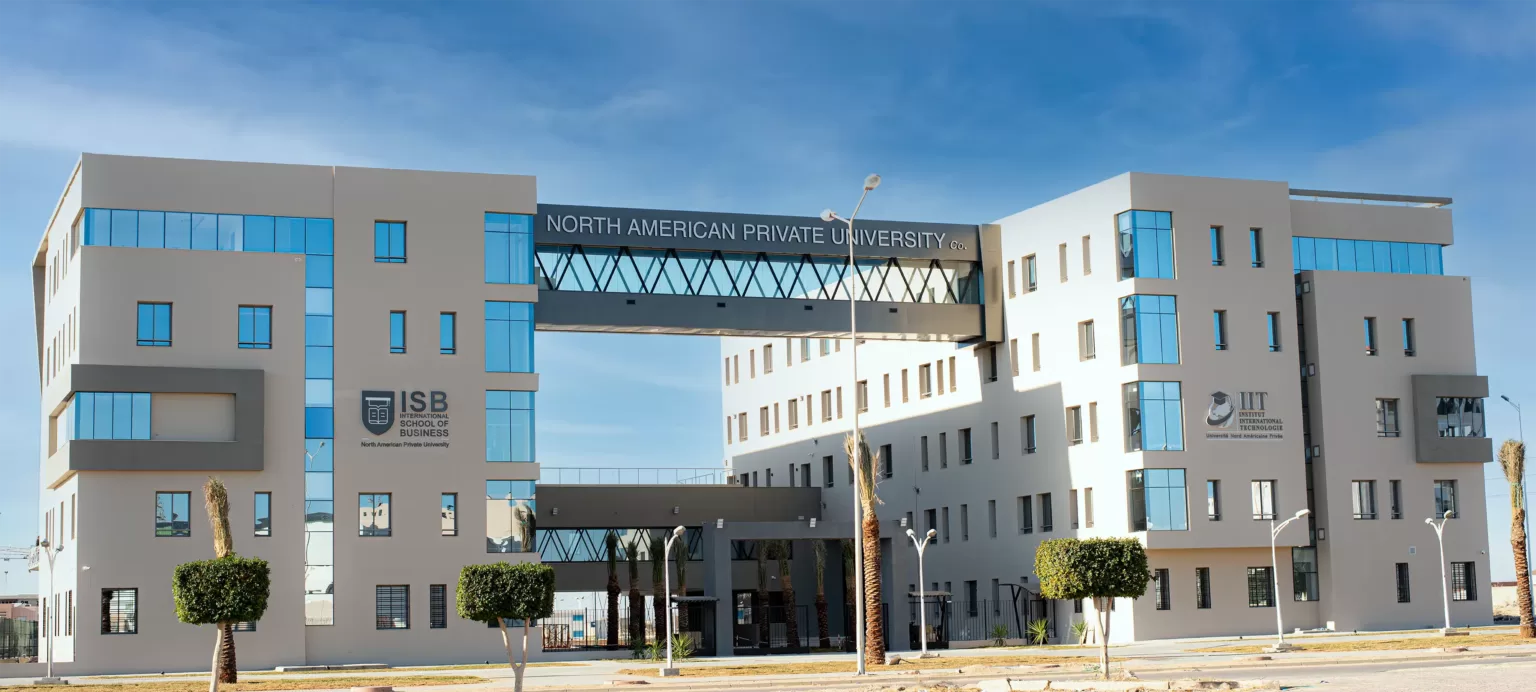
\includegraphics[width=13cm]{images/TemplateImages/Image-Exemple.jpg}}
    \caption{Reception Panel --- Candidate list with year filter}
\end{figure}

\begin{figure}[H]
    \centering
    \fbox{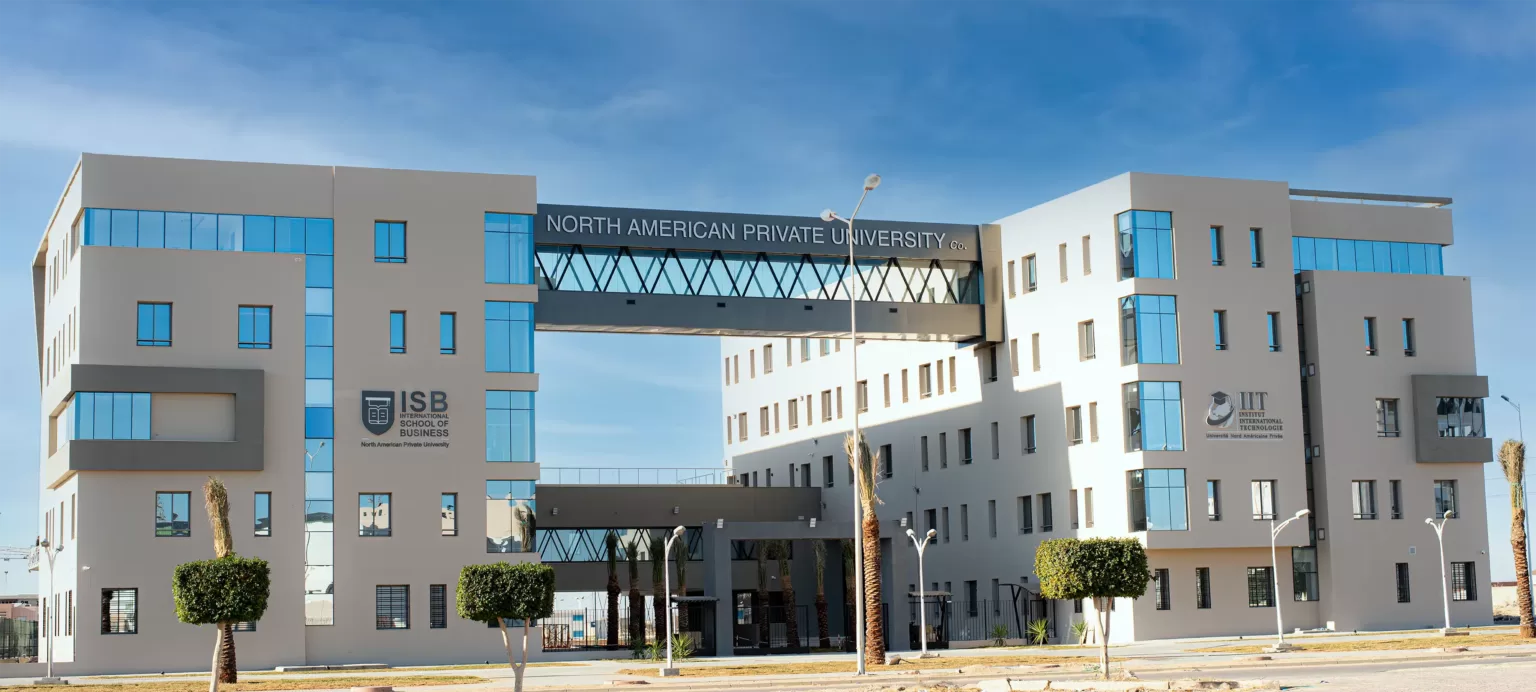
\includegraphics[width=13cm]{images/TemplateImages/Image-Exemple.jpg}}
    \caption{New Candidate registration modal with document upload}
\end{figure}

\section{SPRINT 3 — QUIZ MODULE}

\subsection{Sprint Backlog}
\begin{table}[H]
\centering
\begin{tabular}{|p{1cm}|p{8cm}|p{3cm}|}
\hline
\rowcolor{gray!20}
\textbf{\#} & \textbf{User Story} & \textbf{Status} \\
\hline
12 & As an admin, I want to create quizzes with multiple-choice questions and a time limit & Done \\
\hline
13 & As an admin, I want to assign a quiz to a specific candidate & Done \\
\hline
14 & As a candidate, I want to take my assigned quiz with a visible countdown timer & Done \\
\hline
15 & As a candidate, I want to see my quiz score immediately after submission & Done \\
\hline
16 & As a system, I want to auto-submit the quiz when the time limit is reached & Done \\
\hline
\end{tabular}
\caption{Sprint 3 backlog}
\end{table}

\subsection{Key Technical Implementations}
\begin{itemize}[leftmargin=2cm, topsep=0pt]
    \begin{spacing}{1.25}
        \item \textbf{QuizTimeLimitInterceptor}: A Spring MVC interceptor that blocks quiz submission requests that arrive after the allotted duration.
        \item \textbf{QuizInterface.jsx}: A React component rendering question cards with a real-time countdown timer using \texttt{useEffect} and \texttt{setInterval}.
        \item \textbf{Auto-submit}: When the timer reaches zero, the component automatically calls the submit handler, preventing further answer changes.
        \item \textbf{Score calculation}: \texttt{QuizService.submitQuiz()} iterates over submitted answers, compares them to stored correct answers, and calculates a percentage score.
    \end{spacing}
\end{itemize}

\begin{figure}[H]
    \centering
    \fbox{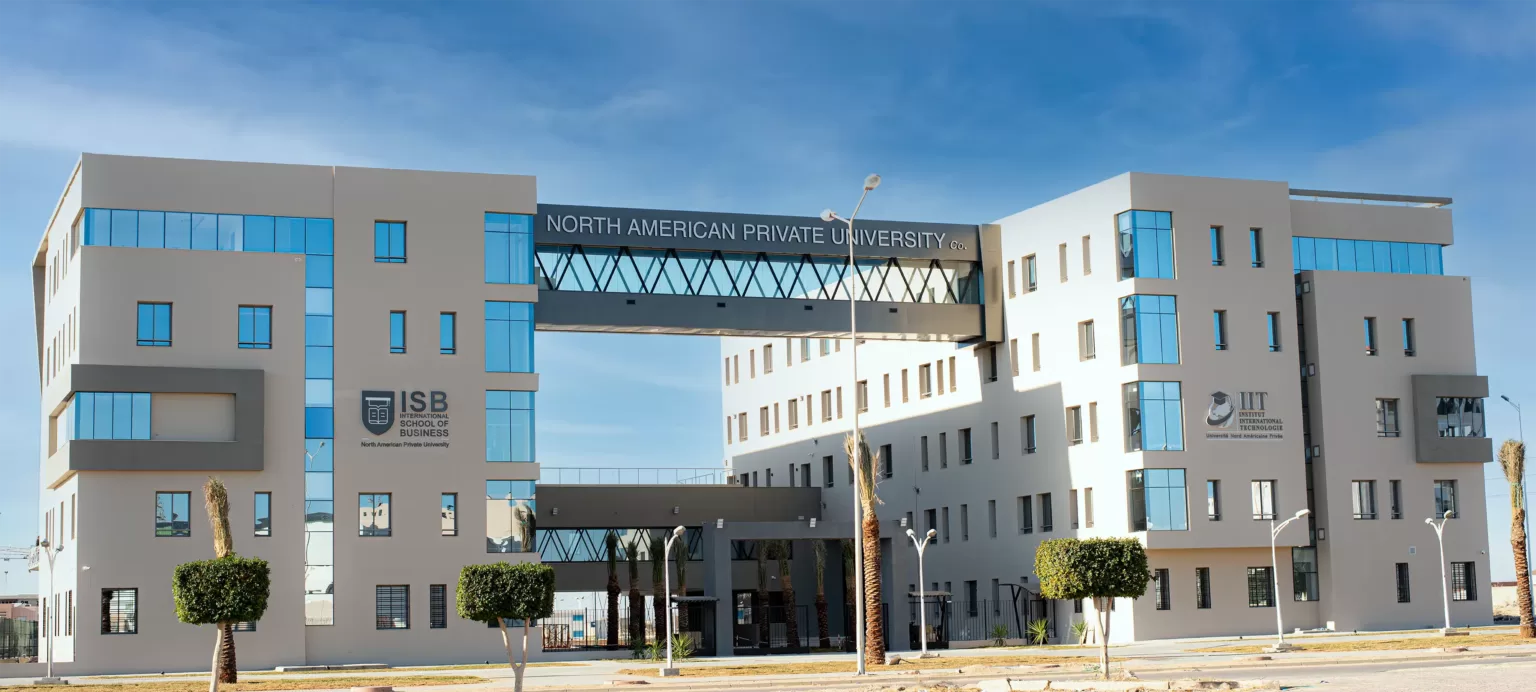
\includegraphics[width=13cm]{images/TemplateImages/Image-Exemple.jpg}}
    \caption{Quiz interface --- Question view with countdown timer}
\end{figure}

\section{SPRINT 4 — AI MODULE AND PROJECT ASSIGNMENT}

\subsection{Sprint Backlog}
\begin{table}[H]
\centering
\begin{tabular}{|p{1cm}|p{8cm}|p{3cm}|}
\hline
\rowcolor{gray!20}
\textbf{\#} & \textbf{User Story} & \textbf{Status} \\
\hline
17 & As a manager, I want the system to rank available projects by relevance & Done \\
\hline
18 & As a manager, I want the system to suggest the best-fit supervisor for each candidate & Done \\
\hline
19 & As a manager, I want to view AI-generated rankings on a dedicated dashboard & Done \\
\hline
20 & As a manager, I want to assign a supervisor to an accepted application & Done \\
\hline
21 & As a manager, I want to conduct interviews and record results & Done \\
\hline
\end{tabular}
\caption{Sprint 4 backlog}
\end{table}

\subsection{Key Technical Implementations}
\begin{itemize}[leftmargin=2cm, topsep=0pt]
    \begin{spacing}{1.25}
        \item \textbf{AiService.rankProjects()}: Scores each available project based on supervisor capacity, project complexity, and application volume. Results are stored as \texttt{AiRanking} records.
        \item \textbf{AiService.matchCandidates()}: For a given supervisor, retrieves all accepted candidates and scores them by specialty alignment, quiz score, and application seniority.
        \item \textbf{AI Insights Dashboard}: A dedicated React page displaying sortable tables of project rankings and candidate matchings fetched from \texttt{GET /api/ai/rankings/**}.
        \item \textbf{Supervisor Assignment}: \texttt{PATCH /api/applications/\{id\}/assign-supervisor} links an accepted application to a chosen supervisor and increments their \texttt{currentInterns} counter.
    \end{spacing}
\end{itemize}

\begin{figure}[H]
    \centering
    \fbox{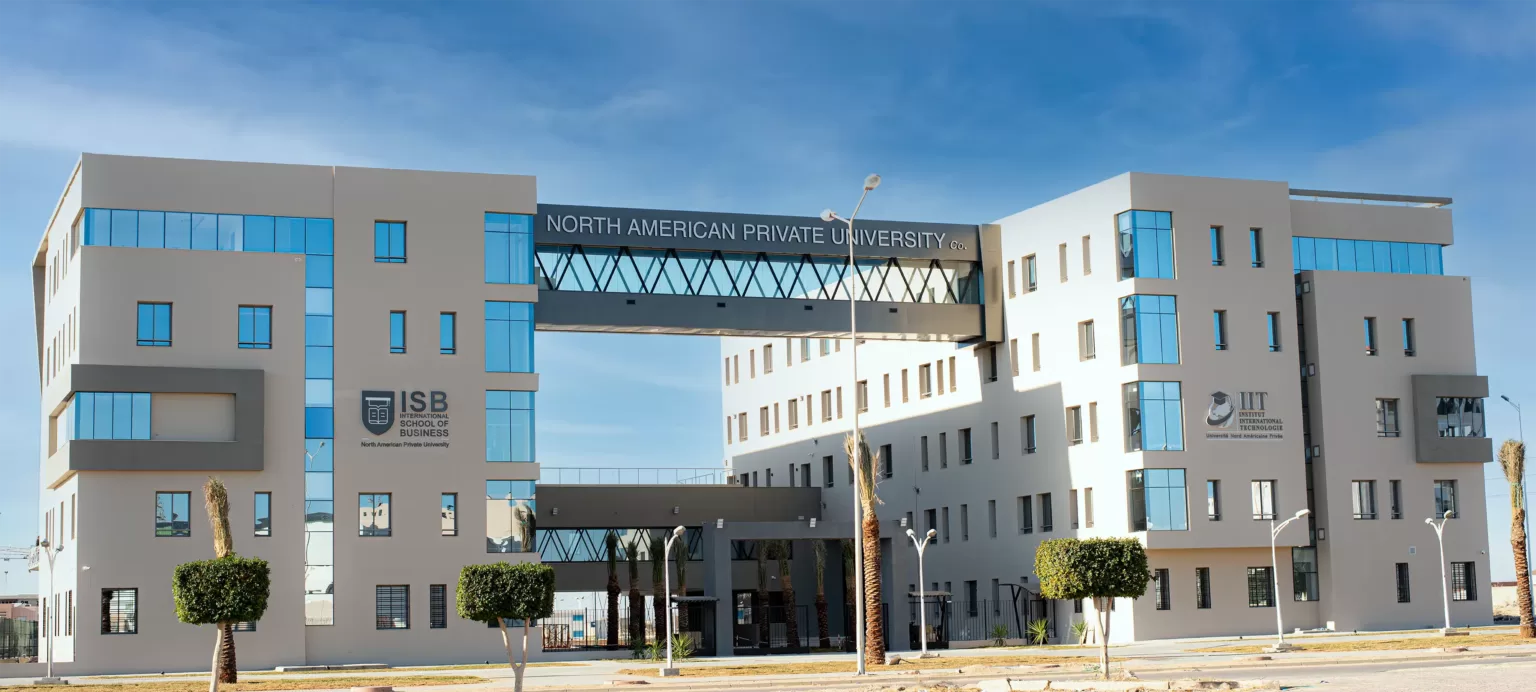
\includegraphics[width=13cm]{images/TemplateImages/Image-Exemple.jpg}}
    \caption{AI Insights page --- Project rankings and candidate matching}
\end{figure}

\begin{figure}[H]
    \centering
    \fbox{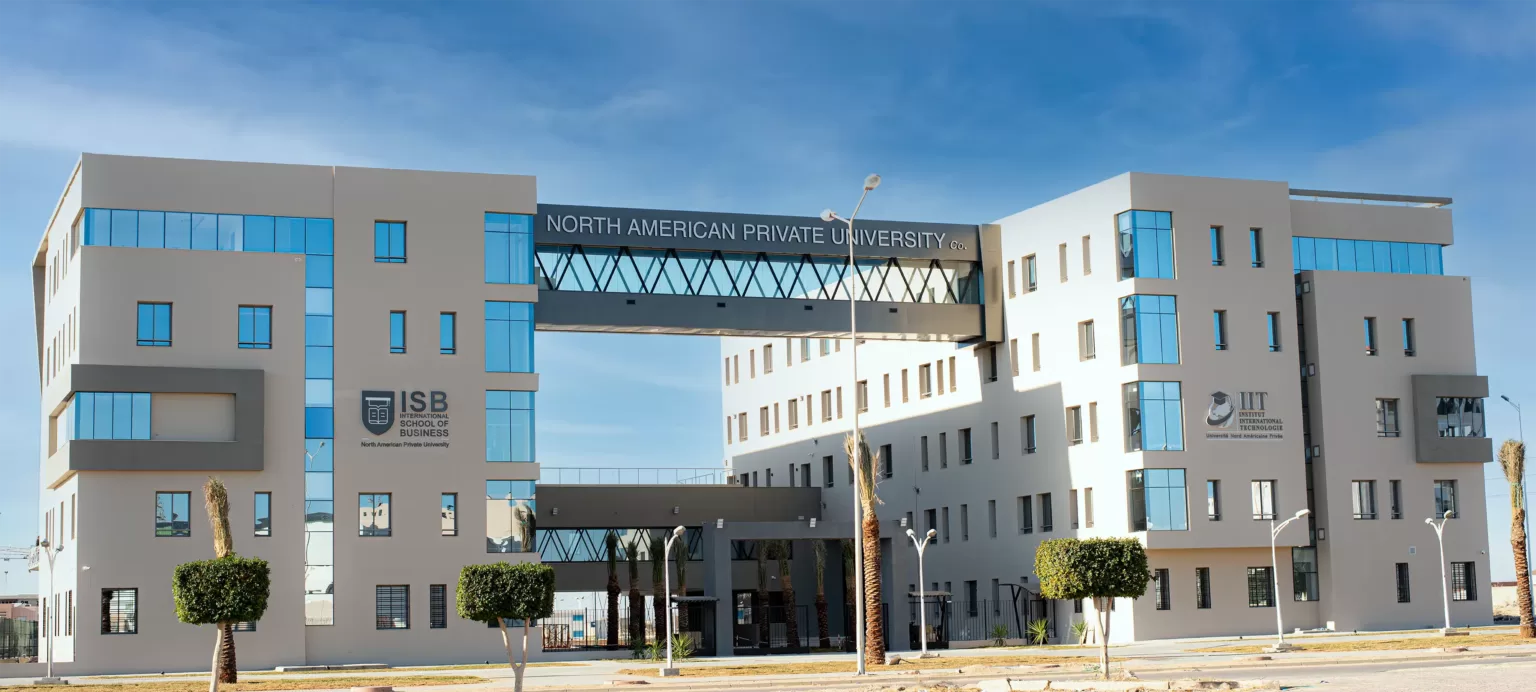
\includegraphics[width=13cm]{images/TemplateImages/Image-Exemple.jpg}}
    \caption{Applications management --- Supervisor assignment workflow}
\end{figure}

\section{CONCLUSION}
This chapter presented the complete implementation of the SIPMS platform across four Scrum sprints. Each sprint delivered functional, tested increments that progressively built the full-featured system. The combination of a robust Spring Boot backend, a reactive React frontend, automated email workflows, and an AI-powered matching engine produces a platform that successfully addresses all the requirements identified in Chapter 2.


    % Chapter 5 — Testing & Validation
    \chapter{TESTING AND VALIDATION}
\begin{spacing}{1.2}
\minitoc
\thispagestyle{MyStyle}
\end{spacing}
\newpage

\section{INTRODUCTION}
This chapter presents the testing strategy adopted to ensure the quality, reliability, and security of the SIPMS platform. We describe the testing methodology, the tools used, and the results obtained for unit, integration, and acceptance testing.

\section{TESTING STRATEGY}
SIPMS was tested using a multi-layered approach covering three levels:

\subsection{Unit Testing}
Individual components (services, controllers, utilities) were tested in isolation using JUnit 5 and Mockito. Key test areas included:

\renewcommand{\labelitemi}{\tiny$\bullet$}
\begin{itemize}[leftmargin=2cm, topsep=4pt]
    \begin{spacing}{1.25}
        \item \textbf{Authentication Service}: Login validation, token generation, role extraction, password hashing.
        \item \textbf{Candidate Service}: CRUD operations, file upload handling, quiz assignment logic.
        \item \textbf{Quiz Service}: Question scoring, attempt management, timer validation.
        \item \textbf{Interview Service}: Scheduling logic, status transitions, result recording.
    \end{spacing}
\end{itemize}

\subsection{Integration Testing}
API endpoints were tested end-to-end using Postman collections. Each endpoint was validated for:
\begin{itemize}[leftmargin=2cm, topsep=4pt]
    \begin{spacing}{1.25}
        \item Correct HTTP status codes (200, 201, 400, 401, 403, 404, 500)
        \item Request validation (missing fields, invalid data types)
        \item Authentication and authorization (RBAC enforcement)
        \item File upload and download flows
    \end{spacing}
\end{itemize}

\subsection{Acceptance Testing}
The platform was validated against the functional requirements defined in the product backlog. Each user story (US-01 to US-21) was tested by simulating real user workflows across all four roles.

\section{TESTING ENVIRONMENT}
\begin{table}[H]
\centering
\begin{tabular}{|p{4cm}|p{9cm}|}
\hline
\rowcolor{gray!20}
\textbf{Component} & \textbf{Tool / Version} \\
\hline
Backend Testing & JUnit 5.10, Mockito 5.11 \\
\hline
API Testing & Postman v11 \\
\hline
Frontend Testing & Chrome DevTools, React DevTools \\
\hline
Database & MySQL 8.0 / H2 (in-memory for tests) \\
\hline
Code Analysis & SonarLint, ESLint \\
\hline
\end{tabular}
\caption{Testing tools and environments}
\end{table}

\section{TEST RESULTS SUMMARY}

\begin{table}[H]
\centering
\begin{tabular}{|p{4cm}|p{3cm}|p{3cm}|p{3cm}|}
\hline
\rowcolor{gray!20}
\textbf{Module} & \textbf{Unit Tests} & \textbf{Integration} & \textbf{Status} \\
\hline
Authentication & 24 & 12 & \textcolor{green}{Pass} \\
\hline
Candidate Management & 18 & 10 & \textcolor{green}{Pass} \\
\hline
Quiz System & 15 & 8 & \textcolor{green}{Pass} \\
\hline
Interview System & 12 & 6 & \textcolor{green}{Pass} \\
\hline
Notifications & 8 & 4 & \textcolor{green}{Pass} \\
\hline
File Upload & 6 & 5 & \textcolor{green}{Pass} \\
\hline
\textbf{Total} & \textbf{83} & \textbf{45} & \textbf{Pass} \\
\hline
\end{tabular}
\caption{Testing results summary}
\end{table}

\section{CONCLUSION}
The testing phase confirmed that all core features of SIPMS function correctly and meet the specified requirements. The system handles edge cases, authentication errors, and invalid inputs gracefully. No critical or high-severity defects were found.



    % Chapter 6 — Discussion & Evaluation
    \chapter{DISCUSSION AND EVALUATION}
\begin{spacing}{1.2}
\minitoc
\thispagestyle{MyStyle}
\end{spacing}
\newpage

\section{INTRODUCTION}
This chapter evaluates the SIPMS platform against the initial objectives defined at the project outset. We discuss the strengths and limitations of the system, analyze the chosen technologies, and propose future enhancements.

\section{EVALUATION OF OBJECTIVES}

\begin{table}[H]
\centering
\begin{tabular}{|p{6cm}|p{4cm}|p{3cm}|}
\hline
\rowcolor{gray!20}
\textbf{Objective} & \textbf{Status} & \textbf{Achievement} \\
\hline
Multi-role authentication with RBAC & Achieved & JWT + Spring Security \\
\hline
Candidate registration and file management & Achieved & Reception Panel \\
\hline
Automated quiz assignment and grading & Achieved & Quiz System \\
\hline
AI-powered project ranking & Achieved & Spring AI Integration \\
\hline
Interview scheduling and result tracking & Achieved & Interview Module \\
\hline
Email notifications & Achieved & JavaMail + Gmail SMTP \\
\hline
Supervisor assignment and capacity management & Achieved & Supervisor Module \\
\hline
\end{tabular}
\caption{Evaluation of project objectives}
\end{table}

\section{TECHNOLOGY EVALUATION}

\subsection{Backend: Spring Boot 3.2 + Java 17}
Spring Boot provided a robust foundation with built-in security, JPA integration, and REST API support. The layered architecture (Controller → Service → Repository) ensured clear separation of concerns and testability.

\subsection{Frontend: React 19 + Vite}
React's component-based model enabled rapid UI development. Vite's fast build times and HMR significantly improved development productivity. Tailwind CSS allowed consistent styling without writing custom CSS.

\subsection{Database: MySQL 8}
MySQL proved reliable for storing structured relational data. Hibernate's DDL auto-update simplified schema evolution during development.

\subsection{AI Integration}
Spring AI provided seamless integration with GPT-4-mini for project ranking and supervisor matching. The AI module operates as a recommendation engine rather than a decision maker, preserving human oversight.

\section{LIMITATIONS}
\begin{itemize}[leftmargin=2cm, topsep=4pt]
    \begin{spacing}{1.25}
        \item \textbf{AI dependency on external API}: The AI module requires a stable internet connection and an active API key. Offline fallback is not implemented.
        \item \textbf{Email delivery reliability}: Gmail SMTP has daily send limits that could be reached in high-volume deployments.
        \item \textbf{File storage}: Currently uses local filesystem storage. A cloud storage solution (AWS S3, MinIO) would be more scalable.
        \item \textbf{Real-time notifications}: The system uses polling instead of WebSockets for in-app notifications, which may introduce slight delays.
    \end{spacing}
\end{itemize}

\section{FUTURE ENHANCEMENTS}
\begin{itemize}[leftmargin=2cm, topsep=4pt]
    \begin{spacing}{1.25}
        \item \textbf{WebSocket integration} for real-time notification delivery
        \item \textbf{Cloud file storage} with AWS S3 or MinIO for better scalability
        \item \textbf{Multi-language support} for international internship programs
        \item \textbf{Advanced analytics dashboard} with charts and exportable reports
        \item \textbf{Mobile application} using React Native for on-the-go access
        \item \textbf{Calendar integration} with Google Calendar / Outlook for interview scheduling
    \end{spacing}
\end{itemize}

\section{CONCLUSION}
The SIPMS platform successfully meets all core requirements defined at the start of the project. While some limitations exist, the system is production-ready and deployed at CLINISYS. The modular architecture allows easy addition of future enhancements.

    
    % General Conclusion
    \chapter*{GENERAL CONCLUSION}
\markboth{\MakeUppercase{GENERAL CONCLUSION}}{}
\addcontentsline{toc}{chapter}{GENERAL CONCLUSION}
\adjustmtc
\thispagestyle{MyStyle}

\par
This final-year project resulted in the successful design and development of \textbf{SIPMS (Smart Internship and Project Management System)}, a comprehensive full-stack web platform built for \textbf{CLINISYS} to digitize and automate the complete internship management lifecycle.

\par
Throughout this project, we addressed a real organizational need: replacing a fragmented, manual internship management workflow with a structured, secure, and intelligent digital platform. The system was built following the \textbf{Scrum agile methodology}, delivering four functional sprints that progressively implemented all required features.

\par
The key achievements of this project are:
\renewcommand{\labelitemi}{\tiny$\bullet$}
\begin{itemize}[leftmargin=2cm, topsep=4pt]
    \begin{spacing}{1.25}
        \item \textbf{Secure multi-role authentication}: A stateless JWT-based system with BCrypt password hashing and fine-grained RBAC enforced across all API endpoints.
        \item \textbf{Automated candidate onboarding}: The Reception Panel allows receptionists to register candidates, upload multiple documents, filter by internship year, and trigger automated welcome emails — all within a single workflow.
        \item \textbf{Objective competency evaluation}: A fully configurable quiz system with a timed interface, automatic scoring, and status management ensures fair and consistent candidate assessment.
        \item \textbf{AI-powered decision support}: Project ranking and candidate-to-supervisor matching algorithms provide managers with data-driven recommendations, reducing subjectivity in assignment decisions.
        \item \textbf{Complete application lifecycle}: From physical reception to final supervised project assignment, every stage of the internship process is tracked, versioned, and auditable.
    \end{spacing}
\end{itemize}

\par
From a technical perspective, this project provided valuable hands-on experience with a modern, production-grade technology stack: \textbf{React (Vite)} for a reactive and accessible frontend, \textbf{Spring Boot (Java 17)} for a robust and scalable backend, \textbf{MySQL} for relational data management, and \textbf{Spring Security + JWT} for enterprise-grade authentication. The integration of \textbf{JavaMail} for automated notifications and \textbf{Spring Multipart} for document management further enriched the technical scope of the project.

\par
Looking ahead, several enhancements could further strengthen the SIPMS platform:
\begin{itemize}[leftmargin=2cm, topsep=4pt]
    \begin{spacing}{1.25}
        \item \textbf{Mobile application}: A React Native or Flutter companion app allowing candidates to track their status and receive push notifications on the go.
        \item \textbf{Advanced AI models}: Replacing the current scoring engine with machine learning models trained on historical internship outcome data to produce more accurate matchings.
        \item \textbf{Electronic signature}: Integrating a digital contract signing module to fully dematerialize the internship agreement workflow.
        \item \textbf{Analytics dashboard}: A management reporting module with visual KPIs tracking acceptance rates, quiz performance distributions, and supervisor workload trends.
        \item \textbf{Docker containerization}: Packaging the entire stack (frontend, backend, database) into Docker Compose for simplified deployment and horizontal scalability.
    \end{spacing}
\end{itemize}

\par
In conclusion, the SIPMS platform successfully delivers on its core objective: transforming a manual, error-prone process into an efficient, transparent, and intelligent system that benefits all stakeholders — from the receptionist registering a candidate on day one, to the manager making a data-informed project assignment decision weeks later. This project stands as a solid foundation for continued digital innovation within CLINISYS.


    % Bibliography
    % ============================================================
%   BIBLIOGRAPHY
% ============================================================
\begin{thebibliography}{99}

\bibitem{spring-boot}
Pivotal Software, \textit{Spring Boot Reference Documentation}, version 3.2,
Available at: \url{https://docs.spring.io/spring-boot/docs/current/reference/html/}, 2024.

\bibitem{spring-security}
Pivotal Software, \textit{Spring Security Reference}, version 6.x,
Available at: \url{https://docs.spring.io/spring-security/reference/}, 2024.

\bibitem{react-docs}
Meta Platforms Inc., \textit{React Documentation},
Available at: \url{https://react.dev/}, 2024.

\bibitem{jwt-spec}
M. Jones, J. Bradley, N. Sakimura, \textit{JSON Web Token (JWT)}, RFC 7519,
Internet Engineering Task Force (IETF), May 2015.

\bibitem{vite-docs}
Evan You, \textit{Vite — Next Generation Frontend Tooling},
Available at: \url{https://vitejs.dev/}, 2024.

\bibitem{mysql-docs}
Oracle Corporation, \textit{MySQL 8.0 Reference Manual},
Available at: \url{https://dev.mysql.com/doc/refman/8.0/en/}, 2024.

\bibitem{hibernate}
Red Hat Inc., \textit{Hibernate ORM Documentation}, version 6.x,
Available at: \url{https://hibernate.org/orm/documentation/}, 2024.

\bibitem{javamail}
Oracle Corporation, \textit{JavaMail API Documentation},
Available at: \url{https://javaee.github.io/javamail/}, 2023.

\bibitem{bcrypt}
N. Provos, D. Mazières, \textit{A Future-Adaptable Password Scheme},
Proceedings of USENIX Annual Technical Conference, 1999.

\bibitem{scrum-guide}
K. Schwaber, J. Sutherland, \textit{The Scrum Guide — The Definitive Guide to Scrum: The Rules of the Game},
November 2020, Available at: \url{https://scrumguides.org/}.

\bibitem{uml-spec}
Object Management Group (OMG), \textit{Unified Modeling Language (UML) Specification}, version 2.5.1,
Available at: \url{https://www.omg.org/spec/UML/}, 2017.

\bibitem{rest-api}
R. Fielding, \textit{Architectural Styles and the Design of Network-based Software Architectures},
PhD Dissertation, University of California, Irvine, 2000.

\bibitem{lucide-react}
Lucide Contributors, \textit{Lucide React — Beautiful \& consistent icon toolkit},
Available at: \url{https://lucide.dev/}, 2024.

\end{thebibliography}


    % Annexes (optional)
    \chapter*{ANNEXES}
\markboth{\MakeUppercase{ANNEXES}}{}
\addcontentsline{toc}{chapter}{ANNEXES}
\adjustmtc
\thispagestyle{MyStyle}

%% add to table of contents : Annexe.1
\makeatletter\renewcommand\thesection{A.\@arabic\c@section}\makeatother

%add spacing in the table of figures
\addtocontents{lof}{\vspace{0.3cm}}

\appendix
\renewcommand{\thefigure}{A.\arabic{figure}}
\setcounter{figure}{0}
\section{TITRE ANNEXE 1}
Lorem ipsum dolor sit amet, consectetur adipiscing elit. Sed non risus. Suspendisse lectus tortor, dignissim sit amet, adipiscing nec, ultricies sed, dolor. Cras elementum ultrices diam. Maecenas ligula massa, varius a, semper congue, euismod non, mi. Proin porttitor, orci nec nonummy molestie, enim est eleifend mi, non fermentum diam nisl sit amet erat. Duis semper. Duis arcu massa, scelerisque vitae, consequat in, pretium a, enim.\par
\begin{figure}[H]%
    \centering
    \fbox{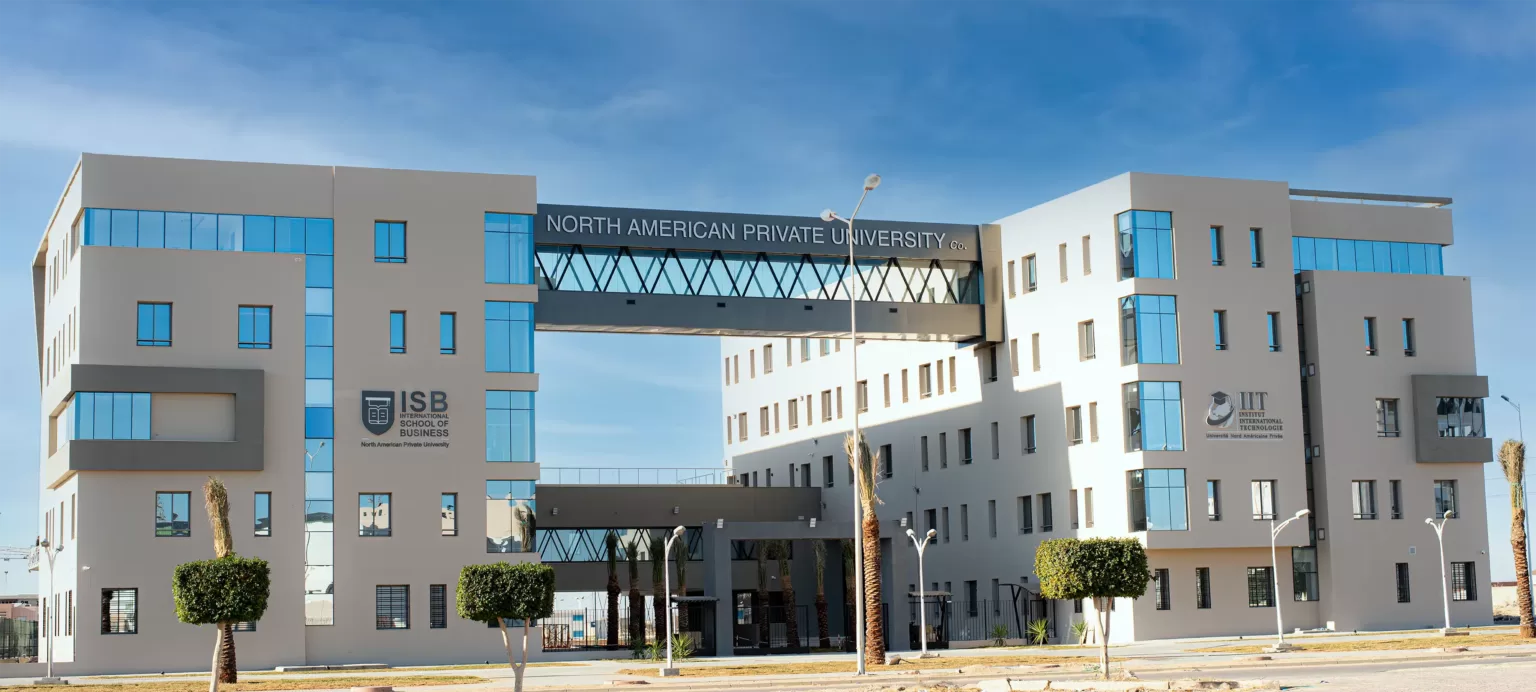
\includegraphics[width=10cm]{images/TemplateImages/Image-Exemple.jpg}}
    \caption{Titre de figure (exemple)}
\end{figure}


    
    % Back cover
    \thispagestyle{empty}
\begin{titlepage}
\begin{center}

%%%%%%%%%%%%%%%%%%%%%%%%%%%%%%%%%%%%%%%%%%%%%%%
% THE HEADER
%%%%%%%%%%%%%%%%%%%%%%%%%%%%%%%%%%%%%%%%%%%%%%%
{%
  \fontsize{9pt}{9pt}\selectfont%
  \begin{tabularx}
    {\textwidth}{ @{} p{0.35\textwidth} @{} p{0.02\textwidth} @{} p{0.3\textwidth} @{} p{0.02\textwidth} @{} p{0.35\textwidth} @{} }
    % line 1
    \centering%
    \begin{spacing}{0.5}
    \noindent
    \end{spacing}
    Ministère de l'Enseignement Supérieur\\% 
    et de la Recherche Scientifique\\%
    \begin{spacing}{1}
    \noindent
    \end{spacing}
    Institut International de Technologie de Sfax\\%
    \begin{spacing}{0.25}
    \noindent
    \end{spacing}
    &%
    % Column 2 is empty 
    &%
    % Column 3
    \centering%
    \multirow{2}{\linewidth}{%
      \centering%
      
\includegraphics[width=4cm, height=2cm]{images/TemplateImages/IIT-Logo.png}%
    }%
    &%
    % Column 4 is empty 
    &%
    % Column 5
    \centering%
    \begin{spacing}{0.25}
    \noindent
    \end{spacing}
    \multirow{2}{\linewidth}{%
      
\includegraphics[width=5.00cm, height=1.80cm]{images/TemplateImages/IIT-Arab.png}%
    }%
    \tabularnewline%
    \arrayrulecolor{black}
    \specialrule{0.75pt}{2pt}{0pt}%
    \specialrule{2.00pt}{1pt}{0pt}%
  \end{tabularx}
}

%%%%%%%%%%%%%%%%%%%%%%%%%%%%%%%%%%%%%%%%%%%%%%%
% THE PAGE CONTENT
%%%%%%%%%%%%%%%%%%%%%%%%%%%%%%%%%%%%%%%%%%%%%%%

\vspace{30pt}

\renewcommand*{\familydefault}{\defaultFont}
  \fontsize{12pt}{12pt}\selectfont%
  \textbf{
  TITRE DU PROJET\\%
  }
\vspace{15pt} {%
  \begin{spacing}{0.05}
    \rule{200pt}{2pt}\\
    \rule{200pt}{0.75pt}\\
  \end{spacing}
  \renewcommand*{\familydefault}{\defaultFont}
  \fontsize{14pt}{14pt}\selectfont%
  \vspace{15pt}
  \textbf{Prénom NOM}
  \vspace{8pt}
  \begin{spacing}{0.05}
    \rule{200pt}{0.75pt}\\
    \rule{200pt}{2pt}\\
  \end{spacing}
}
\end{center}
\vspace{30pt}

%Français
\fontsize{12pt}{12pt}\selectfont%
\underline{\textbf{Résumé:}}\\
Lorem ipsum dolor sit amet, consectetur adipiscing elit. Sed non risus. Suspendisse lectus tortor, dignissim sit amet, adipiscing nec, ultricies sed, dolor. Cras elementum ultrices diam. Maecenas ligula massa, varius a, semper congue, euismod non, mi. Proin porttitor, orci nec nonummy molestie, enim est eleifend mi, non fermentum diam nisl sit amet erat. Duis semper. Duis arcu massa, scelerisque vitae, consequat in, pretium a, enim. Pellentesque congue.\par
\begin{spacing}{1}
\underline{\textbf{Mots clés:}}Lorem, ipsum, dolor, sit amet, consectetur, adipiscing elit.\\
\end{spacing}
\underline{\textbf{Abstract :}}\\
Lorem ipsum dolor sit amet, consectetur adipiscing elit. Sed non risus. Suspendisse lectus tortor, dignissim sit amet, adipiscing nec, ultricies sed, dolor. Cras elementum ultrices diam. Maecenas ligula massa, varius a, semper congue, euismod non, mi. Proin porttitor, orci nec nonummy molestie, enim est eleifend mi, non fermentum diam nisl sit amet erat. Duis semper. Duis arcu massa, scelerisque vitae, consequat in, pretium a, enim. Pellentesque congue.\par
\begin{spacing}{1}
\underline{\textbf{Key-words:}} Lorem, ipsum, dolor, sit amet, consectetur, adipiscing elit.\\
\end{spacing}

\end{titlepage}

\end{document}